

\documentclass[letterpaper,12pt]{article}
\usepackage{tabularx} % extra features for tabular environment
\usepackage{amsmath}  % improve math presentation
\usepackage{graphicx} % takes care of graphic including machinery
\usepackage[margin=1in,letterpaper]{geometry} % decreases margins
\usepackage{ANA-FTAG-2020-08-PAPER-defs}
\usepackage[style=numeric]{biblatex}
\addbibresource{ANA-FTAG-2020-08-PAPER.bib}
\addbibresource{bib/ATLAS.bib}
\addbibresource{bib/ATLAS-useful.bib}
\addbibresource{bib/PubNotes.bib}
\addbibresource{bib/ConfNotes.bib}
\addbibresource{bib/ATLAS-SUSY.bib}
\usepackage[final]{hyperref} % adds hyper links inside the generated pdf file
\usepackage[T1]{fontenc}
\usepackage{setspace}
\usepackage{float}
\usepackage{makeidx}
\usepackage{titlesec}

\newcommand\bjetineq{\mathop{\mbox{$b$-$\mathit{jet}$}}}
\newcommand\bjetunder{\mathop{\footnotesize{\mbox{$b$-$\mathit{jet}$}}}\normalsize}
\newcommand\cjetineq{\mathop{\mbox{$c$-$\mathit{jet}$}}}
\newcommand\cjetunder{\mathop{\footnotesize{\mbox{$c$-$\mathit{jet}$}}}\normalsize}
\setcounter{secnumdepth}{4}

\titleformat{\paragraph}
{\normalfont\normalsize\bfseries}{\theparagraph}{1em}{}
\titlespacing*{\paragraph}
{0pt}{3.25ex plus 1ex minus .2ex}{1.5ex plus .2ex}
\restylefloat*{figure}
\hypersetup{
	colorlinks=true,       % false: boxed links; true: colored links
	linkcolor=blue,        % color of internal links
	citecolor=blue,        % color of links to bibliography
	filecolor=magenta,     % color of file links
	urlcolor=blue         
}

%++++++++++++++++++++++++++++++++++++++++
\linespread{1.17}
\makeindex
\begin{document}


\title{Search for di-Higgs in $bb\tau\tau$ final state using proton-proton collision at $\sqrt{s}$ = 13 TeV data with the ATLAS detector}%Fake Factors Calculation and Implementation in H$\rightarrow$ bb$\tau^+\tau^-$ analysis with MC16a/MC16d in Release 21 with the ATLAS detector
\author{ Zhiyuan Li}
\date{\today}
\maketitle
\begin{figure}[htp]
\begin{minipage}[b]{.5\textwidth}
\centering

\includegraphics[width=1\textwidth]{logo.png}
\end{minipage}\hfill
\begin{minipage}[b]{.45\textwidth}
\vspace{3em}
\centering

\includegraphics[width=1\textwidth]{ATLAS-Logo-Ref-RGB-H_1.jpg}
\end{minipage}
\end{figure}
\newpage


\tableofcontents{}
\printindex{}


\newpage
\section{Flavour tagging at ALTAS}
%test


\subsection{Flavour tagging}


The identification of jets containing $b$-hadrons ($b$-jets) against the large background of jets containing $c$-hadrons ($c$-jets) or coming from the hadronization of light ($u$,$d$,$s$) quarks or gluons is of major importance in many areas of the physics programme of the ATLAS experiment at the LHC. It is crucial in the di-Higgs to $bb\tau\tau$ searches, as well as the recent observation of the Higgs boson decay into bottom quarks \cite{HIGG-2018-04} and of its production in association with a top-quark pair \cite{HIGG-2018-13}, and plays a important role in a large number of Standard Model (SM) precision measurements, studies of the Higgs boson properties, and searches for new phenomena\cite{SUSY-2014-08}, \cite{ATLAS-CONF-2018-043} \cite{Interpreting Higgs result}.

The ATLAS Collaboration uses various algorithms to identify $b$-jets \cite{PERF-2012-04}, referred to as b-tagging algorithms, when analysing data recorded during Run 2 of the LHC. These algorithms exploit the long lifetime, high mass and high decay multiplicity of b-hadrons as well as the properties of the b-quark fragmentation. Given a lifetime of the order of 1.5 ps ($<c\tau>$ $\approx$ 450 $\mu m$), measurable b-hadrons have a significant mean flight length,$<l>$=$\beta\gamma c\tau$, in the detector before decaying, generally leading to at least one vertex displaced from the hard-scatter collision point. The strategy developed by the ATLAS Collaboration is based on a two-stage approach. Firstly, low-level algorithms reconstruct the characteristic features of the $b$-jets via two complementary approaches, one that uses the individual properties of charged-particle tracks, later referred to as tracks, associated with a hadronic jet, and a second which combines the tracks to explicitly reconstruct displaced vertices. These algorithms, first introduced during Run 1 \cite{PERF-2012-04}, have been improved and retuned for Run 2. Secondly, in order to maximise the b-tagging performance, the results of the low-level b-tagging algorithms are combined in high-level algorithms consisting of multivariate classifiers. The performance of a b-tagging algorithm is characterised by the probability of tagging a $b$-jet ($b$-jet tagging efficiency, $\epsilon_b$) and the probability of mistakenly identifying a $c$-jet or a light-flavour jet as a $b$-jet, labelled $\epsilon_c$($\epsilon_l$). 

In this chapter, the performance of the algorithms is quantified in terms of $c$-jet and light-flavour jet rejections, defined as 1/$\epsilon_c$ and 1/$\epsilon_l$, respectively. The imperfect description of the detector response and physics modelling effects in Monte Carlo (MC) simulations necessitates the measurement of the performance of the b-tagging algorithms with collision data \cite{PERF-2012-04 ttbar,b-jet identification semi ttbar}. In this chapter, the measurement of the $b$-jet tagging efficiency of the high-level b-tagging algorithms used in proton–proton (pp) collision data recorded during Run 2 of the LHC at $\sqrt{s}$ = 13 TeV is presented. The corresponding measurements for $c$-jets and light-flavour jets, used in the measurement of the $b$-jet tagging efficiency to correct the simulation such that the overall tagging efficiency of $c$-jets and light-flavour jets match that of the data, are described elsewhere \cite{ATLAS-CONF-2018-006}, \cite{cjet}. The production of $t\bar{t}$ pairs at the LHC provides an abundant source of $b$-jets by virtue of the high cross-section and the $t \rightarrow Wb$ branching ratio being close to 100\%. A very pure sample of $t\bar{t}$ events is selected by requiring that both $W$ bosons decay leptonically, referred to as di-leptonic $t\bar{t}$ decays in the following. Similarly a source of $c$-jets can be obtained by requiring that one $W$ boson decay leptonically and the other decay hadronically, referred to as semi-leptonic $t\bar{t}$ decay in the following. 


% The identification of the jets originating from the hadronization of heavy-flavour quarks is made possible by the distinctive properties of the heavy hadrons produced in the process. For instance, the large life time of $b$-quarks allows them to travel a measurable distance from the primary interaction point before to decay, giving rise to displaced tracks which can form secondary vertices. The ATLAS Collaboration developed several algorithms to identify (tag) the jets from $b$-quark hadronization based on the properties detailed above. 

The most performant algorithms presently in use in physics analyses at ATLAS are based on multivariate (MV2) combinations of the available information or a deep feed-forward neural network(DL1)\cite{tagging}\cite{ATL-PHYS-PUB-2017-013}, as shown in Figure \ref{fig:MV2_DL1}. Depending on the low-level algorithm, the DL1 tagger can be further separated into two taggers: DL1 and DL1r, where the DL1 tagger uses traditional track-based impact parameter taggers IP2D and IP3D and DL1r tagger uses a Recurrent Neural Network tagger (RNNIP)\cite{ATL-PHYS-PUB-2017-013}. The DL1r tagger is now the default b-tagging algorithm used for flavour tagging in ATLAS.
%Their high mass also leads to decay products with a larger transverse momentum relative to the jet axis with respect to the ones typically found in jets from light partons. Finally, heavy hadrons have a sizable branching ratio for semileptonic decays, hence the presence of soft leptons in the produced jets provides another tool for heavy jet identification. %The general strategy is to start with simple algorithms that exploits a particular property of b jets and progressively add more information to build moresophisticated algorithms. %The output of these algorithms consists in a discriminant value for each jet. Operating points are then defined as thresholds on the discriminant, designed to provide a determined efficiency for identifying b jets.
% Low-level $b$-taggingalgorithms fall into two broad categories. A first approach, implemented in the IP2D and IP3D algorithms \cite{ATL-PHYS-PUB-2017-013}, or RNNIP \cite{ATL-PHYS-PUB-2017-003} is inclusive and based on exploiting the large impact parameters of the tracks originating from the $b$-hadron decay. The second approach explicitly reconstructs displaced vertices. To maximise the $b$-tagging performance, low-level algorithm results are combined using multivariate classifiers. To this end, two high-level tagging algorithms have been developed. The first one,MV2\cite{ATL-PHYS-PUB-2017-013}, is based on a boosted decisiontree (BDT) discriminant, while the second one,DL1, is based on a deep feed-forward neural network(NN). These two algorithms are presented in fig .
\begin{figure}
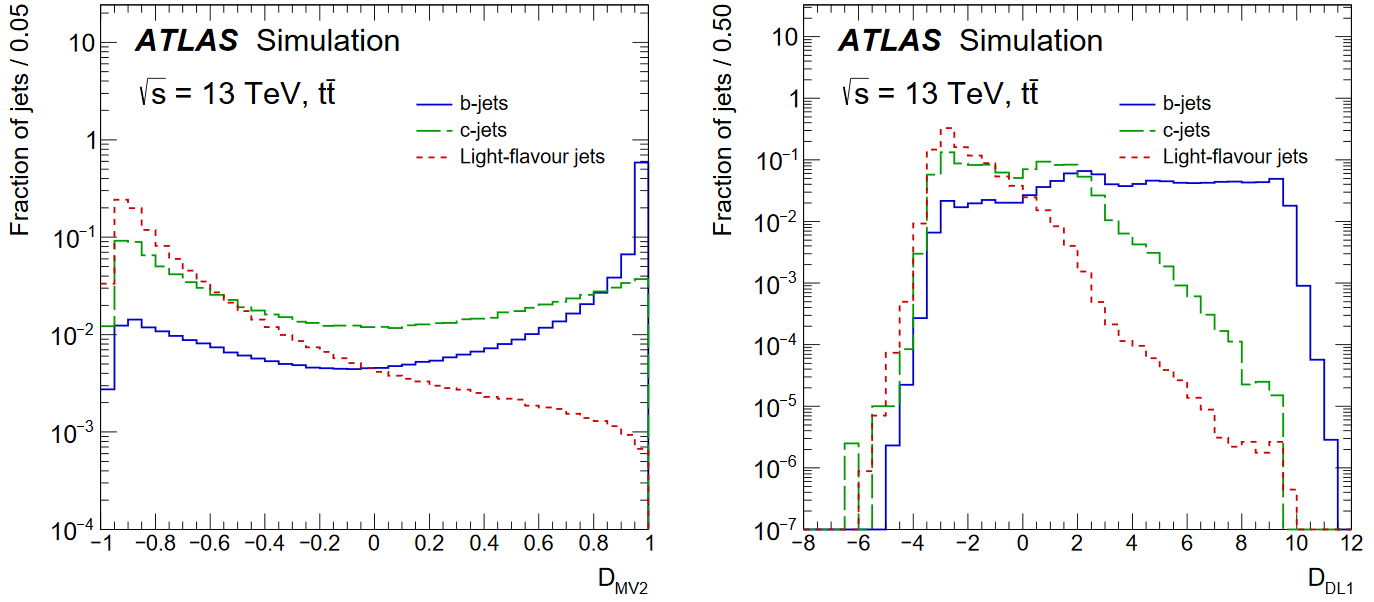
\includegraphics[width=1\textwidth]{MV2_DL1.png}
\caption{Performance of MV2c10 and DL1 tagger\cite{FTAG-2018-01}.}\label{fig:MV2_DL1}
\end{figure}

\subsection{Calibration methods}
Monte Carlo (MC) simulations are not able to model very well the performance of the $b$-tagging algorithms in data. For this reason calibration is required, i.e. correcting MC to match the data in terms of $b$-tagging efficiency, charm-jet mis-tagging and light-jet mis-tagging rates\cite{FTAG-2018-01}. The calibration is done for all supported working points, which are cuts in the b-tagging algorithm output identifying the tagging efficiencies, and jet collections(TODO: refer back to the object definition chapter). In general, the efficiency is calculated with data and simulations, and scale factors are then calculated to match the efficiency extracted from simulations to the data. More details of the calibrations of different flavour are given in the following subsections.


For the \bjet\  calibration, the performance of the $b$ tagging algorithms is evaluated in the simulation and the efficiency with which these algorithms identify jets containing $b$-hadrons is measured in collision data. The measurement uses a likelihood-based method in a di-leptonic (both $W$ bosons from the top decay decay into leptons) $t\bar{t}$ sample of highly enriched in $t\bar{t}$ events. Events with 2 jets and 2 opposite signs leptons are selected from di-leptonic $t\bar{t}$ samples. The data $b$-jet efficiency is then extracted from a combined likelihood fit, and subsequently compared with that predicted by the simulation. Scale factors are then calculated to match the performance of the algorithms to the data\cite{FTAG-2018-01}.

For the light jet mis-tagging calibration, two methods are used to measure the mistagging rate from the data: the negative tag method, which uses a high statistics data sample enriched in light-jets with the application of a modified algorithm which reverses some of the criteria used in the nominal identification algorithm, and the adjusted Monte Carlo (adjusted-MC) method, which adjust the characteristic track observables in the simulation to match the data, and then compares the adjusted simulation to the "standard" simulation. The scale factors are then calculated using the these two methods. The scale factors of the two different methods are in good agreement within the systematics uncertainties\cite{ATLAS-CONF-2018-006}. 
%The aim of this calibration is to calibrate $b$-jets that have been mis-tagged as light-jets of b-tagging algorithm. As the $b$-tagging algorithm is very efficient in rejecting light-jets, the light-jet fraction is enriched via "flipped" taggers, which negates the sign of track IP parameters before $b$-tagging\cite{ATLAS-CONF-2018-006}. The calibrations of the standard and the 'flipped' tagger are assumed to be equal. The calibration is extracted using the leading $p_T$ jet of Z+jets events using a 2D fit. TODO: cite the light-jet tagging Int note
%light-jet fractions in the $b$-like region are too low,  The Z + jets events are then selected, the secondary vertex mass is fitted to obtain flavour fractions and perform a likelihood fit to extract light-jet mistag rate.

The charm-jet mis-tagging calibration utilises semi-leptonic $t\bar{t}$ events. The events kinematics are shown by the diagram in Figure \ref{fig:feynman}, where the $t\bar{t}$ pair decays to a pair of $b$ and $\bar{t}$ quark, circled in red. One of the $W$ boson, circled in blue, decays hadronically to quarks, and the other $W$ boson, decays leptonically to either electron or muon and the corresponding neutrinos, circled in purple and green. The lepton in the final state is used for triggering, and a combined likelihood fit is used to extract the $c$ mis-tagging efficiency (more details in Section \ref{charm mistagging}). 

\begin{figure}[H]
\centering
\begin{minipage}[b]{.45\textwidth}
\centering
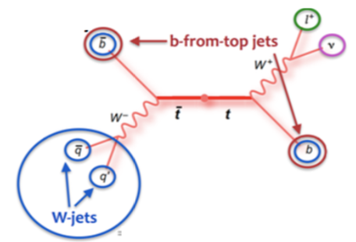
\includegraphics[width=1\textwidth]{feynman.png}
\end{minipage}
\caption{Feynman diagram of the semi-leptonic $t\bar{t}$ events.}
\label{fig:feynman}
\end{figure}
\section{Charm mis-tagging calibration}
\label{charm mistagging}
\subsection{Introduction}
%As Shown in Fig \ref{fig:feynman}, the calibration uses the semi-leptonic $t\bar{t}$ events, which one $W$ boson from top decays leptonically to a charged lepton and neutrino and one $W$ decays hadronically and dominantly to a charm and a strange quark, among other pairs.
As determined by the CKM matrix\cite{CKM1}\cite{CKM2}, the $W$ boson decay to light-quark pair or light quark $c$ quark pair dominantly, and very rarely decay to pairs containing $b$-quarks. More specifically, the branching ratio of a $W$ boson decays to a pair of light quarks or a light quark and a $c$ quark is 33.7\%, and of pairs containing a b quark is only 0.058\%\cite{PDG}. Therefore, $b$-tagged jets from the $W$ decay are most likely to be mis-tagging of $c$-jets or light-jets. Given the ratio between the DL1 light-jet rejection and the corresponding charm-jet rejection ranges from 10 to 40 (see ref\cite{ATL-PHYS-PUB-2017-013}), the $c$-jet in $c$-jet-light-jet pairs is the most likely source for the $b$-tagged jet. A kinematic likelihood technique, referred to as KLFitter\cite{ERDMANN201418}, is used to assign jets to the proper $t\bar{t}$ decay product without using any $b$-tagging information (more details in Section \ref{KLFitter}). The charm-jet efficiency is then extracted by a combinatorial likelihood fit applying to the pair of jets from $W$ decays, where the main floating parameter is the $c$-jet efficiency\cite{cjet}. 

It is worth mentioning that my qualification task to become an ATLAS author is to calibrate the rate of a charm jet being mis-identified as a $b$-jet, which is a part of the calibration of the $b$-tagging algorithm. The calibration uses the full Run2 data of 139 fb$^{-1}$ integrated luminosity collected at $\sqrt{s}$ = 13 TeV by the ATLAS detector. In the task, 4 rounds of calibration has been conducted, each round with different jet collection and b-tagging algorithm. To be concise only the result of the last round is presented in this chapter. During the task the calibration range has been extended down to 20 GeV (which was 25 GeV) and a new selection category has been developed to increase the stats of the scale factors in the high $p_T$ ($p_T$ greater than 70 GeV) region.

\subsection{Data and Monte Carlo samples}
%%%%%%%%%%%%%%%%%%%%%%%%%%%%%%%%%%%%%%%%%%%%%%%

\label{sec:samples}
%%%%%%%%%%%%%%%%%%%%%%%%%%%%%%%%%%%%%%%%%%%%%%%
The data analysed in this study correspond to 139~fb$^{-1}$~\cite{DAPR-2010-01,DAPR-2011-01,DAPR-2013-01,LUCID2}, of \(pp\)
collision data collected by the ATLAS detector between 2015 and 2018
with a centre-of-mass energy of 13~\TeV\ and a 25\,ns proton bunch
crossing interval. 
The data sample was collected using 
a set of single-muon~\cite{Aad:2020uyd} and single-electron 
triggers~\cite{TRIG-2018-05}.
The single-muon triggers had \pt\ thresholds in the range of 20--26~\GeV\ for 
isolated muons and 50~\GeV\ for muons without any isolation requirement. 
The single-electron triggers employed a range of \pt\ thresholds in the range 24--300~\GeV\ 
and a combination of quality and isolation requirements depending on the 
data-taking period and the \pt\ threshold.
%The uncertainty in the combined 2015--2018
%integrated luminosity is 1.7\%~\cite{ATLAS-CONF-2019-021}, obtained
%using the LUCID-2 detector~\cite{LUCID2} for the primary luminosity
%measurements. 
 All detector subsystems were required to be operational
during data taking and to fulfil data quality requirements.  


The $t\bar{t}$ samples and the single top-quark in the Wt and s-channel samples are generated with the {\tt Powheg-Box} v2 \cite{powheg} generator. Electroweak t-channel single top-quark events are generated using the {\tt Powheg-Box} v1 generator. The parton shower, fragmentation, and the underlying event are simulated using {\tt Pythia} 6.428\cite{pythia} with the CTEQ6L1 PDF sets and the corresponding Perugia 2012 tune (P2012)\cite{perugia}. The top-quark mass is set to 172.5 GeV. The {\tt EvtGen} v1.2.0 program \cite{evtgen} is used to model the properties of the bottom and charm hadron decays. The $t\bar{t}$ production cross-section is calculated at NNLO+NNLL (next-to-next-to-leading-logarithm)\cite{NNLO}. For single-top processes, the generator NLO cross-sections are used. Events containing $W$ or $Z$ bosons with associated jets are simulated using {\tt Sherpa} 2.2.1\cite{sherpa}. All $W$/$Z$+jets events are normalised to the predicted cross-sections using NNLO calculations. All samples are passed through the full GEANT4\cite{GEANT4} simulation of the ATLAS detector and are reconstructed with the same software as used for data.

\subsection{Kinematic Likelihood Fitter}
\label{KLFitter}
Top quarks decay to a $W$ boson and a bottom quark in nearly 100\% of all cases. Consequently, the final state of a top-quark pair is characterised by the decay products of the two $W$ bosons. %If one of the $W$ bosons decays into a charged lepton and a neutrino while the other one decays into a pair of quarks, the decay mode is referred to as the single-lepton, or semi-leptonic decay mode. 
The fraction of top-quark pairs decaying either in the single-electron or single-muon decay mode is about 30\%. The corresponding event signature is defined by exactly one electron or muon, four jets out of which two contain a $b$-hadron, and a large amount of missing transverse momentum due to the un-detected neutrino. The Kinematic Likelihood Fitter\cite{ERDMANN201418}, is a reconstruction technique developed to reconstruct $t\bar{t}$ decays, which exploits the above decay topology of the top quark in the semi-leptonic channel in order to properly associate jets to the quarks in the final state of the decay process. In the semi-leptonic decay of the $t\bar{t}$ system, the resulting tree level situation contains two $b$-quarks from the top quark decays, and two light or charm quarks from the $W$ boson decay (Figure \ref{fig:feynman}). A likelihood is used to properly assign these four jets to the true decay quarks. The leading order scenario is assumed, giving rise to four jets in the final $t\bar{t}$ decay topology, two of which are $b$-jets. Three of the jets in the decay are associated to the hadronic top decay, whereas a final fourth jet along with the charged lepton and neutrino build the leptonic top\cite{cjet}.


\subsubsection{Maximising likelihood}
Taking only four jets in the event limits the total number of possible jet orderings (permutations) in the event. In the semi-leptonic channel, four jets can be permuted a total number of times equal to 4! = 24. However, the two jets (from light or $c$-quarks) resulting from the hadronic $W$ decay are kinematically indistinguishable. This reduces the possible number of permutations to 12. Furthermore, no $b$-tagging information is used in the kinematic likelihood to limit the possible number of permutations.
For every combination of jet ordering the likelihood is maximised over its free parameters, the energy of the four jets, the lepton energy and the three components of the momentum of the neutrino, and provides a value based on how closely the kinematic information from the reconstructed objects for a specific jet ordering resembles the expected kinematic behaviour of the decay of a Standard Model semi-leptonic $t\bar{t}$ event. The likelihood therefore distinguishes the possible permutations on an event-by-event basis. The best permutation, given by the largest log-likelihood value, is adopted as the jet ordering for the event\cite{cjet}. To improve the purity of the selected events further, an additional requirement of log-likelihood > -48  is placed on the output of the likelihood value for the chosen event permutation. An example of the distribution of log-likelihood of the best permutations is shown in Figure \ref{fig:loglikelihood}.

\begin{figure}[H]
\centering
\begin{minipage}[b]{.45\textwidth}
\centering
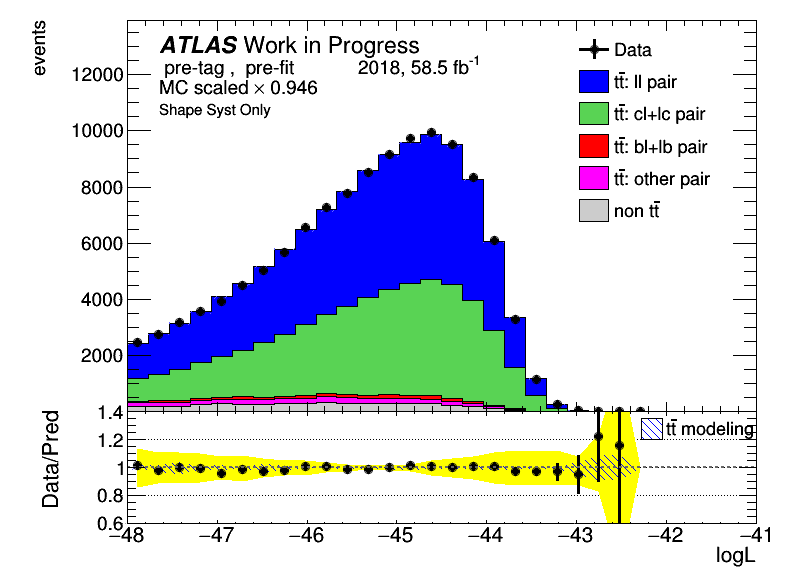
\includegraphics[width=1\textwidth]{Distribution_March/DataMC_LLR.png}
\end{minipage}
\caption{Log-likelihood distribution of the best permutations.}
\label{fig:loglikelihood}
\end{figure}
% \subsubsection{Extracting efficiencies}

% The measurement of the $c$-jet $b$-tagging efficiency is performed using decays of $W$ boson to a pair of quarks with at least one of them having charm flavour. The branching ratio of hadronic $W$ decays to at least one charm quark and another quark (either s or d or very rarely b) is predicted to be 0.5 in the Standard Model due to the CKM unitarity\cite{CKM1}\cite{CKM2}. Given that there are two jets from the hadronic $W$ decay, the $c$-jet component corresponds to a fraction of exactly 25 \% of any jets from $W$ boson decays. 
% The $c$-jet tagging efficiency is extracted from the fraction of selected di-jet pairs containing exactly one $b$-tagged jet. Given that the ratio between the DL1 light-jet rejection and the corresponding $c$-rejection ranges from 10 to 40 (see Ref.\cite{ATL-PHYS-PUB-2017-013}) the $c$-jet in cl pairs is the most likely source for the tagged jet.

% The compositional jet fraction as a function of jet pT and $p_{T}$ is shown in Figure 3 prior to requiring any $b$-tagging for the two jets assigned to the $W$-boson decay and after the log likelihood requirement. With increasing jet $p_{T}$, contributions other than from $W$ boson decay are suppressed and the $c$-jet fraction asymptotically reaches 25 \% of the jets assigned as originating from the hadronic $W$-boson.
% \subsection{low-$p_{T}$ extension}
% Instead of requiring exactly 4 jets with $p_{T}$ greater than 25 GeV, the events are now required to have exactly 3 jets with $p_{T}$ greater than 25 GeV and exactly 1 jet with $p_{T}$ greater than 20 GeV. 

% \subsection{ high-$p_{T}$ selection}



% \subsection{samples and data}

% \subsubsection{MC samples}


% \subsubsection{data samples}
\subsubsection{KLFitter Jet selection}
In the standard selection, only events with exactly 4 jets are selected. Therefore, there is no room for wrong choice of choosing 4 jets out of 4 jets, which will then be the input for the KLFitter tool (More details can be found in section \ref{standard selection}). However, this becomes a problem when the 4 jets requirement is lifted. In the selection for reducing errors in high-$p_{T}$ bins of scale factors (referred to as high-$p_{T}$ selection from now on, more details can be found in section \ref{high_pt_selection}), events with at least 5 jets can also pass the selection. Therefore how to choose the 4 jets out of the 5 jets and possibly more jets is now a problem. Without using any b-tagging information, the best solution in this case would be to simply select the 4 jets with the highest $p_T$. %In the June 2019 Charm calibration and calibrations before that, the 'kBtagPriorityFourJets' selection mode was used, which will select the 4 jets highest $p_T$ while prioritising the $b$-jets. This was not a problem until the high-$p_{T}$ selection was introduced. With this particular mode an anomaly was observed in the $b$-jet purity in the reconstructed $W$ boson decay jets, when comparing the combination of the high-$p_{T}$ selection and the standard selection to the standard selection, as shown in Figure \ref{fig:highpt}(a)(b). 
To check the impact of including more then 4 jets in the events, the $b$-jet purity was checked, which is defined as:
\begin{equation}
\bjetineq purity= \frac{N_{true\ \bjetunder}}{N_{all}},
\end{equation}
where $N_{true \bjetunder}$ stands for the number of events with a true $b$-jet from the $W$ decay, and $N_{all}$ stands for the number of all events.
%This was due to the $b$-jets being given higher priority in jet selection. To resolve this problem, from the calibration in December 2019 and after, the selection mode will be switched to 'kLeadingFour' selection mode, which selects the 4 jets with the highest $p_T$. 
%Using this mode avoids using $b$-tagging information in the jet selection stage, and gives equal priority to all jets entering the selection. The huge anomaly in $b$-jet purity has disappeared after switching to the 'KLeadingFour' mode (Figure \ref{fig:highpt}(c)(d)),
As shown in Figure \ref{fig:highpt}(a)(b), less $b$-jets are presented in the high-$p_{T}$ selection. This difference can be reduced after applying $b$-tagging of jets passing DL1r at 60\% working point as shown in Figure \ref{fig:highpt}(c)(d). The $b$-jet purity after $b$-tagging is defined as:
\begin{equation}
\bjetineq\ purity\ after\ tagging= \frac{N_{true\ tagged\ \bjetunder}}{N_{tagged}},
\end{equation}
where $N_{true\ tagged\ \bjetunder}$ stands for the number of events with a true tagged $b$-jet from the $W$ decay, and $N_{tagged}$ stands for the number of events with a tagged $b$-jet from the $W$ decay.
\begin{figure}[H]
%\begin{minipage}[b]{.45\textwidth}
\centering
%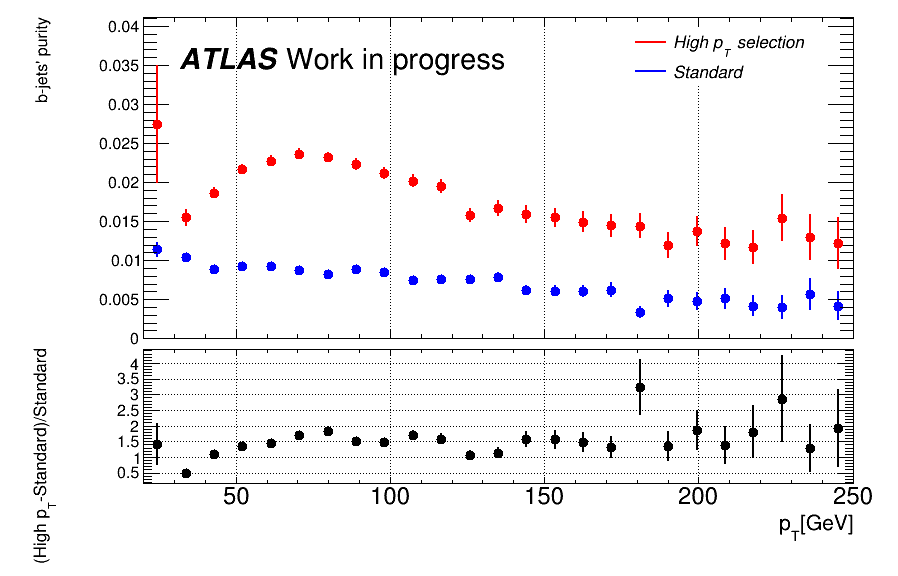
\includegraphics[width=1\textwidth]{statsplot_thesis_standard_anomaly/_stats_bjets_purityp_Tjet0GeV.png}
%\footnotesize (a) Anomaly in the leading jet $b$-jet purity due to the selection mode 'kBtagPriorityFourJets'.
%\end{minipage}\hfill
%\begin{minipage}[b]{.45\textwidth}
%\centering
%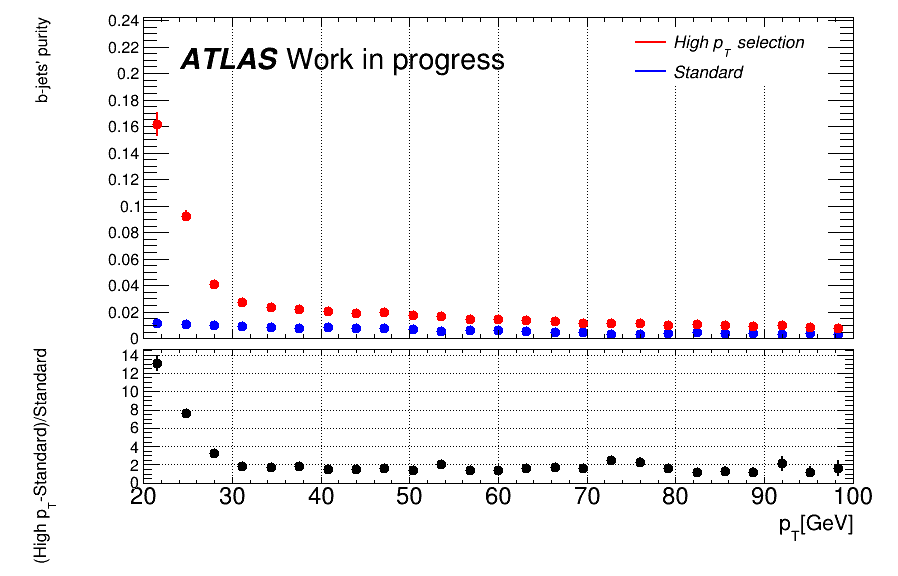
\includegraphics[width=1\textwidth]{statsplot_thesis_standard_anomaly/_stats_bjets_purityp_Tjet1GeV.png}
%\footnotesize (b) Anomaly in the sub-leading jet $b$-jet purity due the selection mode 'kBtagPriorityFourJets'.
%\end{minipage}\hfill
\begin{minipage}[b]{.45\textwidth}
\centering
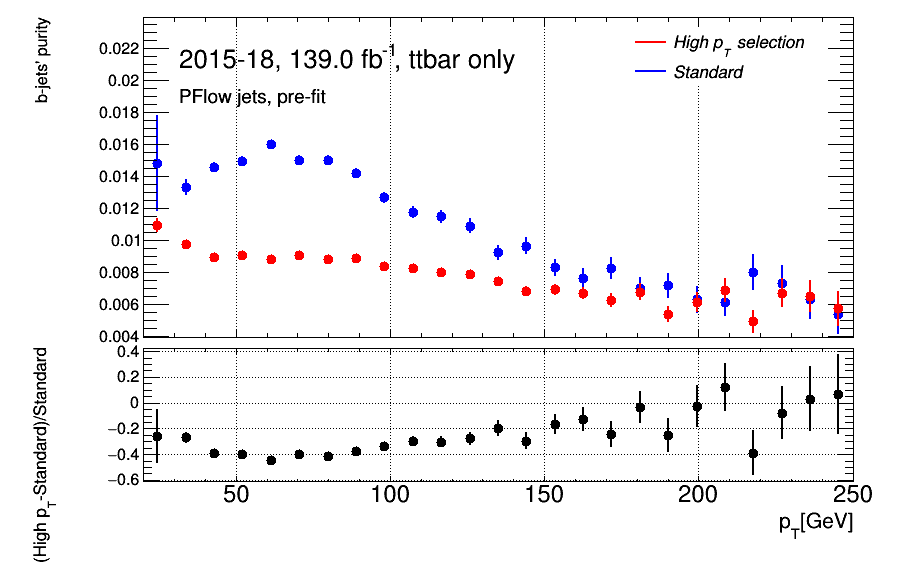
\includegraphics[width=1\textwidth]{b_purity/_stats_bjets_purityp_Tjet0GeV.png}
\footnotesize (a) Comparing the leading jet $b$-jet purity distribution between the standard selection and the high $p_T$ selection.\label{fig:b_after_leading}
\end{minipage}\hfill
\begin{minipage}[b]{.45\textwidth}
\centering
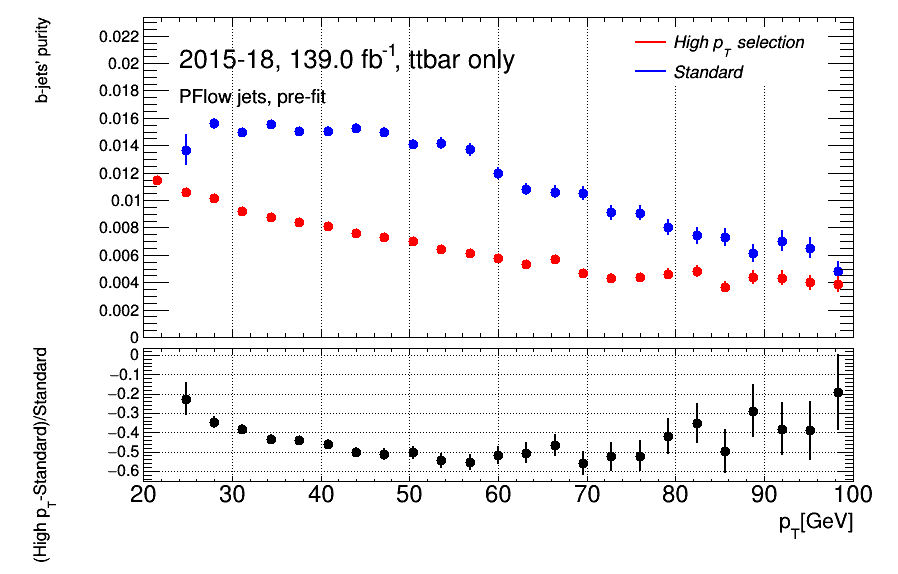
\includegraphics[width=1\textwidth]{b_purity/_stats_bjets_purityp_Tjet1GeV.png}
\footnotesize (b) Comparing the sub-leading jet $b$-jet purity distribution between the standard selection and the high $p_T$ selection.\label{fig:b_after_subleading}
\end{minipage}\hfill
\begin{minipage}[b]{.45\textwidth}
\centering
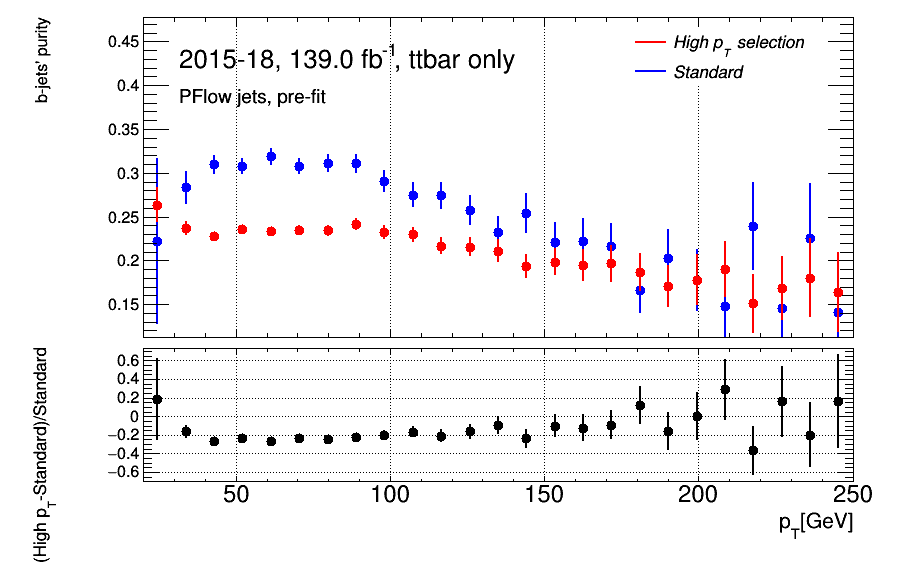
\includegraphics[width=1\textwidth]{b_purity/tagged_stats_bjets_purityp_Tjet0GeV.png}
\label{b_tagged_leading}
\footnotesize (c) Comparing the leading jet $b$-jet purity distribution between the standard selection and the high $p_T$ selection after applying $b$-tagging with DL1r tagger at 60\% working point.
\end{minipage}\hfill
\begin{minipage}[b]{.45\textwidth}
\centering
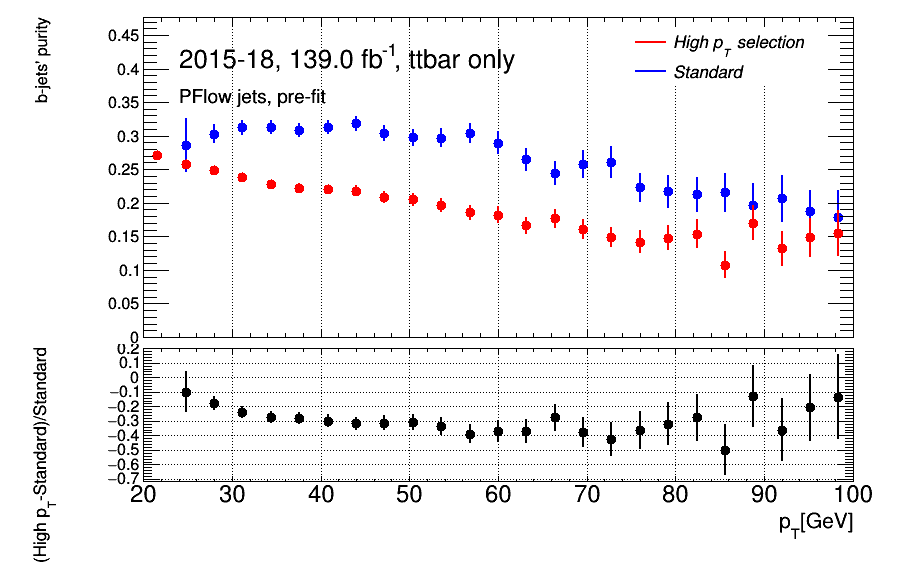
\includegraphics[width=1\textwidth]{b_purity/tagged_stats_bjets_purityp_Tjet1GeV.png}
\label{b_tagged_subleading}
\footnotesize (d) Comparing the sub-leading jet $b$-jet purity distribution between the standard selection and the high $p_T$ selection after applying $b$-tagging with DL1r tagger at 60\% working point.
\end{minipage}
\caption{Comparison of the $b$-jet purity in leading (the left column) and sub-leading (the right column) jet $p_{T}$ distribution.}
\label{fig:highpt}
\end{figure}

\subsection{Event selection}
\label{Event selection}
 % The analysis uses the full available integrated luminosity collected with the ATLAS detector from the all years. This corresponds to a collected luminosity of 139 fb$^{-1}$. The event selection aims to select a sample enriched in $t\bar{t}$ events. The lowest un-prescaled single electron and single-muon triggers are used.


\subsubsection{Standard selection}
\label{standard selection}
Events are required to contain exactly one trigger-matched lepton with $p_{T}$ above 27 GeV and exactly four jets with $p_{T}$ above 25 GeV. Leptons are required to have $p_{T}$ above 27 GeV in order to avoid the turn-on curve for the single lepton triggers. Events which contain an additional lepton with $p_T$ above 27 GeV are rejected. Of these four jets, at least two must be $b$-tagged using the DL1 $b$-tagger at 60\% working point (this will not bias the calibration result as these two $b$-jets are then assigned to the top decay, which is not used for extracting the efficiency). In addition, events are required to have a minimum of 20 GeV missing transverse momentum, which is assumed to be the result of the neutrino from the leptonically decaying $W$ boson. For each event, the kinematic likelihood fitter is applied which determines the jet assignment to the various top decay products assumed from the $t\bar{t}$ decay products. An additional requirement of log-likelihood > -48  is placed on the output of the likelihood value for the chosen event permutation. Due to the requirement on jet $p_T$ and binning strategy, the calibration result can be applied to jets with $p_{T}$ between 25 to 200 GeV. The yields of the data/MC are given in Table \ref{tab:yields_standard}, and the kinematic distributions before any tagging or fitting and after the standard selection are shown in appendix, Figure \ref{fig:standard_selection}.

 \begin{table}[h]
 \begin{centering}
 \begin{tabular}{c|c|c}
          \hline
          \hline
Sample &  Yield & Error \\ \hline   \hline      
Data   & 118729.0& N/A\\ \hline
$t\bar{t}$  & 120908.0 &$\pm$134.6\\ \hline
Other  &   4621.5 &$\pm$91.9\\ \hline
Data/MC&  0.946   &$\pm$0.003\\ \hline

 \end{tabular} 
 \caption{Yields of the data and MC samples of 2018 dataset before tagging after standard selection. The uncertainty only includes the MC statistical component.} \label{tab:yields_standard}
 \end{centering}

 \end{table}








\subsubsection{Selection for low-$p_{T}$ extension}
In order to extend the calibration in the low-$p_{T}$ region so that the calibration can be applied to jets with $p_{T}$ smaller to 25 GeV, instead of requiring events to have exactly 4 jets, events are required to have exactly 3 jets with $p_{T}$ greater than 25 GeV and exactly 1 jet with $p_{T}$ greater than 20 GeV. Other than that, all other requirements for the selection are the same. The distributions of the sub-leading jet are shown in appendix, Figure \ref{fig:lowpT_selection}. Good agreement between MC and data is shown in these distributions, and the $p_{T}$ range of the sub-leading has gone down to 20 GeV. The scale factors are shown in the appendix in Figure \ref{fig:lowpT3}. The range of the calibration is then extended with jet $p_{T}$ down to 20 GeV. 




\subsubsection{High $p_T$ selection}
\label{high_pt_selection}
Instead of requiring events to have exactly 4 jets, events are required to have at least 5 jets with $p_{T}$ greater than 25 GeV, in which at least 1 jet with $p_{T}$ greater than 70 GeV. The choice of cut value is based on study shown in the following section \ref{cutvalue}. Other than that, all other requirements for the selection are the same.  The kinematics distributions are shown in the appendix, Figure \ref{fig:highpT_selection}. 

 \begin{table}[h]
 \begin{centering}
 \begin{tabular}{c|c|c}
          \hline
          \hline
Sample &  Yield & Error \\ \hline   \hline      
Data   &  160749.0 & N/A\\ \hline
Ttbar  &  164234.8 &$\pm$156.4 \\ \hline
Other  &    5408.2 &$\pm$92.5 \\ \hline
Data/MC&   0.948   &$\pm$ 0.003 \\ \hline
 \end{tabular} 
 \caption{Yields of the data and MC samples of 2018 dataset before tagging after the combination of the standard selection and the high-$p_T$ selection. The uncertainty only includes the MC statistical component.} \label{tab:yields_highpT}
 \end{centering}
 \end{table}

\paragraph{Optimisation of high $p_{T}$ cut}
\label{cutvalue}

In the high-$p_{T}$ selection, the value to define high-p$_{T}$ is chosen to be 70 GeV. A study has been done to investigate the effect on the $c$-jet purity and the potential statistical gain, where the $c$-jet purity is defined as:
\begin{equation}
\cjetineq\ purity = \frac{N_{true\ \cjetunder}}{N_{all}},
\end{equation}
where $N_{true\ \cjetunder}$ stands for the number of events with a true $c$-jet from the $W$ decay, and $N_{all}$ stands for the number of all events. 
The $c$-jet purity and the statistical gain are calculated for 4 different cut values as shown in Figure \ref{fig:cutvalue}, comparing with the cut value of 0. The value of 70 GeV is chosen because of its relatively small effect on the $c$-jet purity and relatively high gain in statistics. 


\begin{figure}
\begin{minipage}[b]{.45\textwidth}
\centering
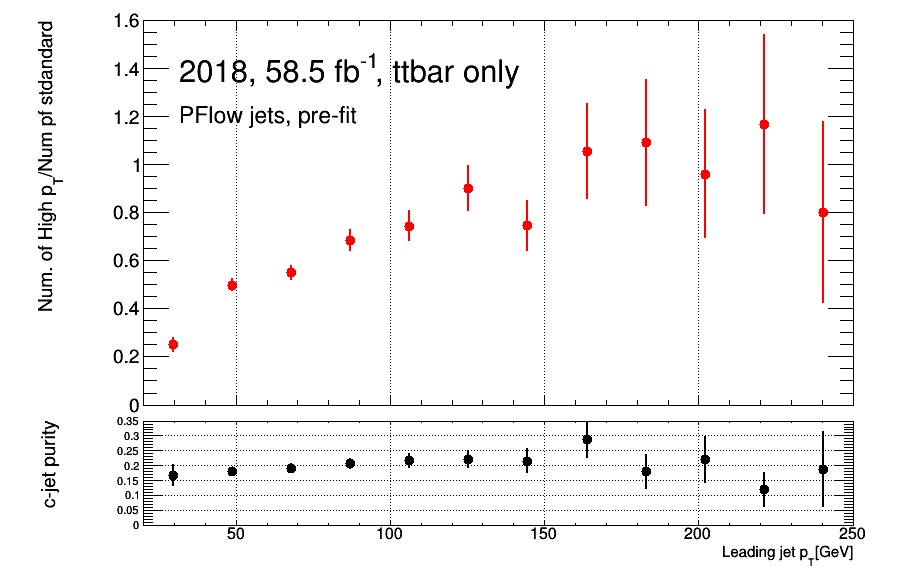
\includegraphics[width=1\textwidth]{stat_gains/statsgain_0GeV.png}
\footnotesize (a) Gain in stats and the $c$-jet purity with cut value 0 GeV.
\end{minipage}\hfill
\begin{minipage}[b]{.45\textwidth}
\centering
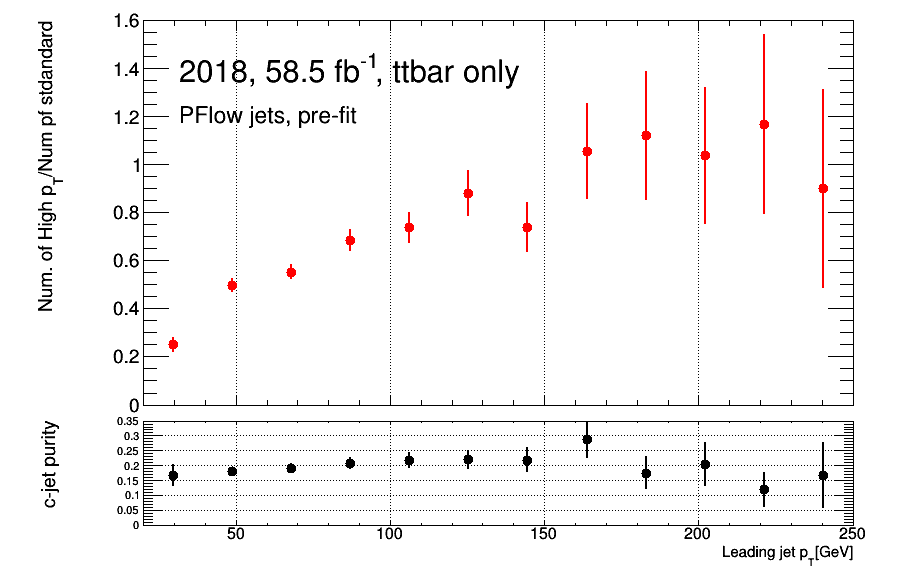
\includegraphics[width=1\textwidth]{stat_gains/statsgain_40GeV.png}
\footnotesize (b) Gain in stats and the $c$-jet purity with cut value 40 GeV.
\end{minipage}\hfill
\begin{minipage}[b]{.45\textwidth}
\centering
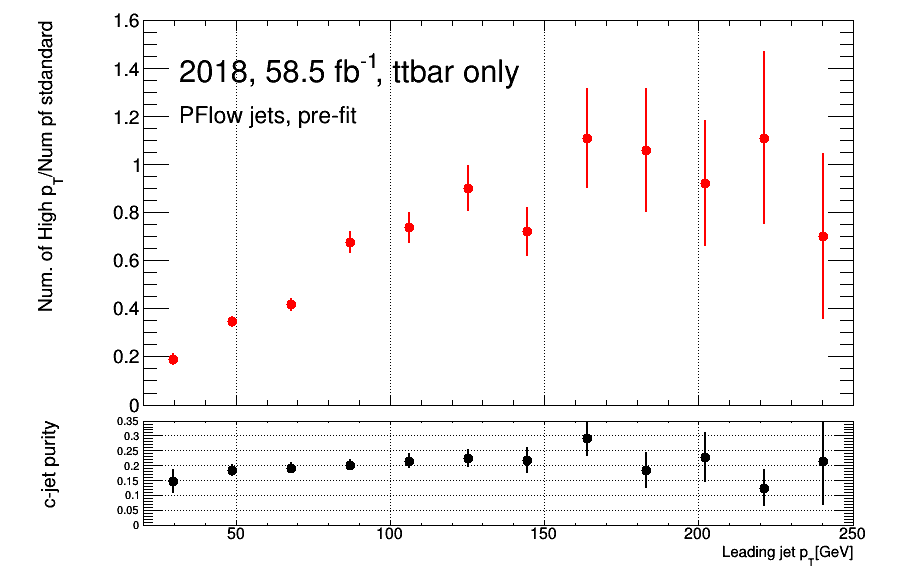
\includegraphics[width=1\textwidth]{stat_gains/statsgain_70GeV.png}
\footnotesize (c) Gain in stats and the $c$-jet purity with cut value 70 GeV.
\end{minipage}\hfill
\begin{minipage}[b]{.45\textwidth}
\centering
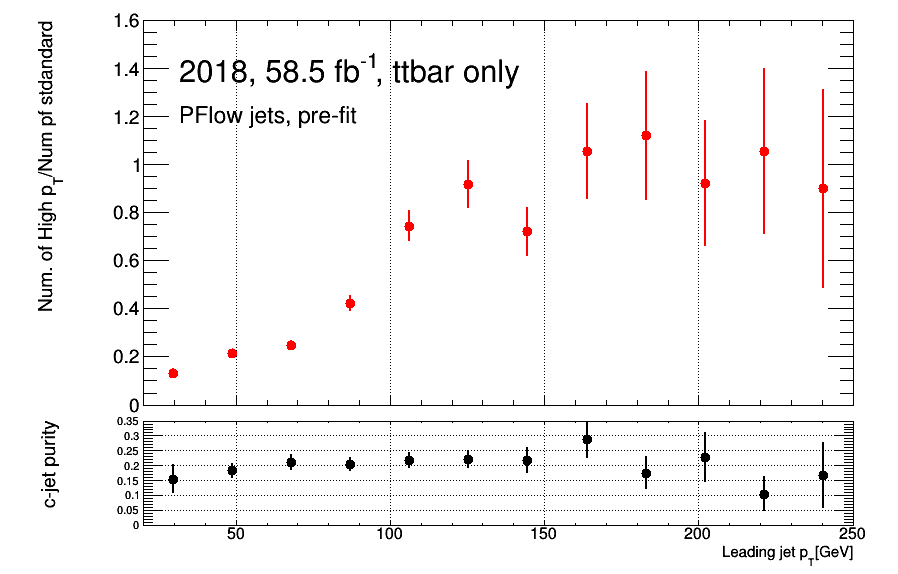
\includegraphics[width=1\textwidth]{stat_gains/statsgain_90GeV.png}
\footnotesize (c) Gain in stats and the $c$-jet purity with cut value 90 GeV.
\end{minipage}\hfill
\begin{minipage}[b]{.45\textwidth}
\centering
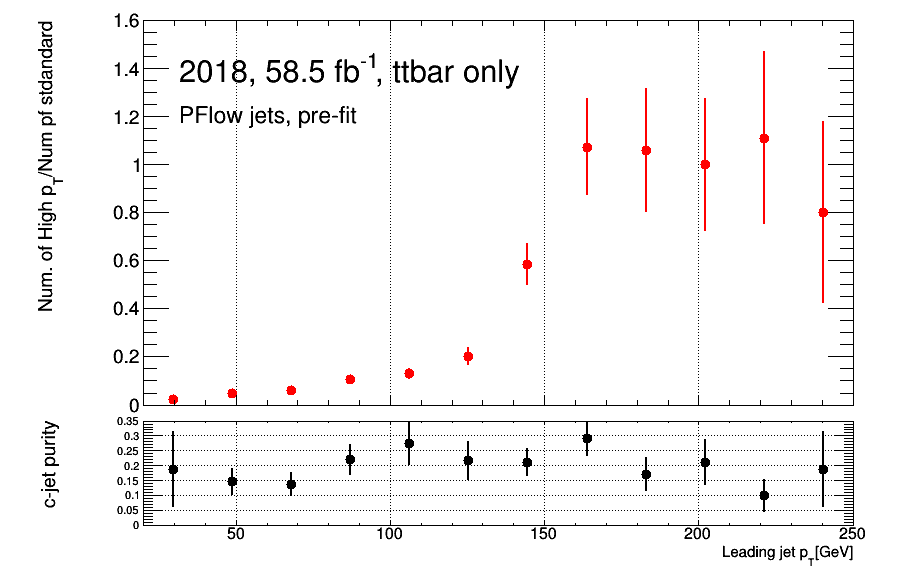
\includegraphics[width=1\textwidth]{stat_gains/statsgain_140GeV.png}
\footnotesize (d) Gain in stats and the $c$-jet purity with cut value 140 GeV.
\end{minipage}\hfill

\caption{Comparison of different cut values in terms of gain in stats and $c$-jet purity.}
\label{fig:cutvalue}
\end{figure}


\subsection{Systematic uncertainties}

The systematic uncertainties considered and propagated in this calibration can be broadly categorised into experimental systematics and modelling uncertainties. Supporting material for this section can be found in the appendix, Tab.\ref{tab:systematics}.
\subsubsection{Experimental uncertainties}

Experimental uncertainties are related to the detector and estimated using MC simulations. The electron energy scale and resolution are corrected to provide better agreement between MC predictions and data, uncertainties due the corrections are considered. Uncertainties are taken into account the electron trigger, identification and reconstruction efficiencies, and for uncertainties associated with the isolation requirements. Scaling and smearing corrections are applied to the $p_T$ of simulated muons in order to minimise the differences in resolution between data and MC events, and the uncertainties of the corrections are considered. Differences in the identification efficiency and in the efficiency of the trigger selection are also taken into account. The jet energy scale (JES) uncertainty depends on $p_T$ and $\eta$ and takes into account uncertainties due to pile-up effects. Uncertainties on the jet energy resolution (JER) is taken into account. 'Category Reduction' is used for JES uncertainties which include the necessary uncertainties for combination. Uncertainties on the energy scale and resolution of the electrons, muons, jets and taus are propagated to the calculation of the $E_T^{miss}$, which also has additional dedicated uncertainties on the scale, resolution, and reconstruction efficiency of tracks not associated to any of the reconstructed objects, along with the modelling of the underlying event. Uncertainties on the $b$-tagging probabilities for $b$- and light-jets are considered both for the tagging jets assigned to the $b$-quark from top decay and for the jets associated to the hadronically decaying $W$ boson.
%The uncertainty on these corrections is taken into account as a shape-dependent systematic uncertainty in the final fit of the backgrounds and signal models.

\subsubsection{Modelling uncertainties} Uncertainties on the modelling of the inclusive $t\bar{t}$ background are estimated by replacing the nominal MC sample by alternative MC samples. The nominal sample is also replaced by variations of the matrix element generator, parton shower, and initial and final state radiation. In all cases, MC-to-MC SFs are taken into account. The uncertainty in the choice of NLO matrix element generator is derived by comparing two alternative predictions, {\tt POWHEG} and {\tt aMC@NLO\_MG5}, each of which is showered with {\tt HERWIG++}. An uncertainty due to the choice of parton shower and hadronisation model is derived by comparing the prediction from {\tt POWHEG} interfaced either to {\tt PYTHIA8} or {\tt HERWIG++}. Finally, the uncertainty on modelling of initial and final state radiation is assessed with two alternative {\tt POWHEG+PYTHIA8} samples. The samples include one with an increase in radiation which has the re-normalisation and factorisation scales decreased by a factor of two and the \textit{hdamp} parameter doubled, while the sample with a decrease in radiation has the scales increased by a factor of two.

\subsubsection{Under-estimation of $t\bar{t}$ + Heavy flavour background }
The $b$-jets are rarely found in the two $W$ decay jets. There are two main sources of the $b$-jets, first is a $W$ boson decaying to pair of $b$ and $c$ quark. The other source is when the $t\bar{t}$ plus a gluon process is selected, and the gluon is split into a pair a $b$ quarks. If we require no $c$-jet in either top-decay jets or $W$-jets, the only main source of the $b$-jets in the $W$-jets is the $t\bar{t}$ + heavy flavour process. It's shown in for the both PFlow and VR-Track jets collections, this process is underestimated by the MC by about 30\%, as shown in Table \ref{tab:3byields1}, \ref{tab:3byields2} and Figure \ref{fig:3bplots}. A precise measurement in another analysis shows that this factor is 1.25 \cite{ttbar+HF SF}. Therefore a 1.25 $\pm$ 0.25 scale factor is applied to all events with 3 truth $b$ jets, and all results shown in the following have this scale factor implemented. 
\begin{table}[]
    \centering
    \begin{tabular}{c|c}
        Data & 1589.0 \\
         $t\bar{t}$ & 1102.7 $\pm$ 12.5 \\
         Other & 82.7 $\pm$ 5.5 \\
         Data/MC & 1.341 $\pm$ 0.037 \\
    \end{tabular}
    \caption{Yields of the 2018 data/MC, combining the standard and te high $p_T$ selection with at least 1 PFlow $W$ jet with DL1r > 8 to reject most of the light and $c$ jets.}
    \label{tab:3byields1}
\end{table}

\begin{table}[]
    \centering
    \begin{tabular}{c|c}
        Data & 1336.0 \\
         $t\bar{t}$ & 943.5 $\pm$ 11.6 \\
         Other & 69.1 $\pm$ 4.5 \\
         Data/MC & 1.319 $\pm$ 0.040 \\
    \end{tabular}
    \caption{Yields of the 2018 data/MC, combining the standard and te high $p_T$ selection with at least 1 VR-Track $W$ jet with DL1r > 8 to reject most of the light and $c$ jets.}
    \label{tab:3byields2}
\end{table}

\begin{figure}
    \centering
    \begin{minipage}[b]{.45\textwidth}
\centering
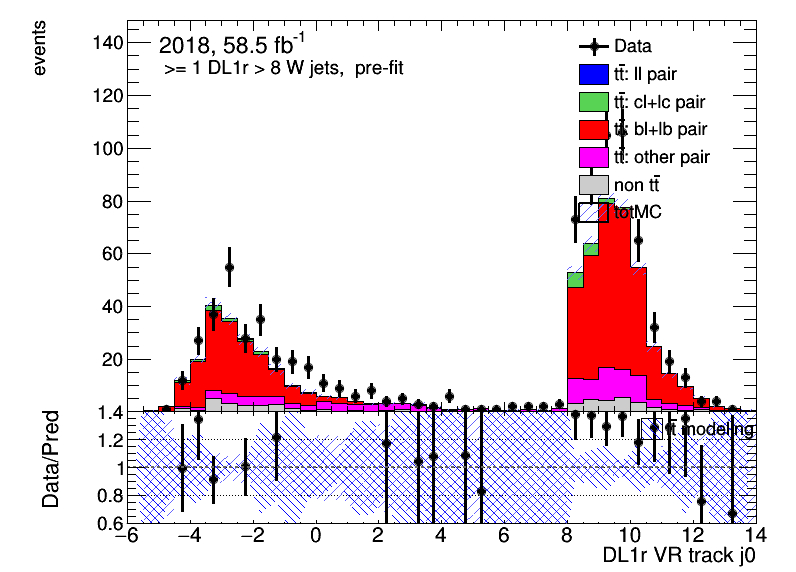
\includegraphics[width=1\textwidth]{3bplots/3bplots.png}
\end{minipage}
    \caption{The DL1r score distribution of the leading VR-Track jet, requiring at least 1 VR-Track jets have DL1r > 8 to reject most of the light and the $c$ jets, with $t\bar{t}$ modelling and stats uncertainties. }
    \label{fig:3bplots}
\end{figure}


\subsection{Results}
\label{result}


\subsubsection{Overview}
Four rounds of calibrations have been carried out, containing different jet collections, Monte Carlo samples, analysis framework and $b$-jet identification algorithm. In the latest round, the calibration includes the EMPFlow jet and VR-Track jet collection, and MV2c10, DL1 and DL1r taggers. Each calibration is carried out with all supported jet collections and taggers, with the full data set collected from 2015 to 2018 in the ATLAS detector. The low-$p_T$ selection and the standard selection are carried out for all four calibrations, while the high-$p_T$ selection is only implemented in the latest calibration. 

\subsubsection{Kinematic distributions}
The kinematic distributions of the MC and the data of the latest calibration (October 2020) are shwon in Figure \ref{fig:taggers_PFlow}, \ref{fig:jets_PFlow}, \ref{fig:angles_PFlow}, \ref{fig:mass_PFlow} for the PFlow jets and Figure \ref{fig:taggers_VRJets}, \ref{fig:jets_VRJets}, \ref{fig:angles_VRJets}, \ref{fig:mass_VRJets} for the VR-Track jets, combining the standard selection and the highest $p_T$ selection. 

\begin{figure}[H]
\begin{minipage}[b]{.45\textwidth}
\centering
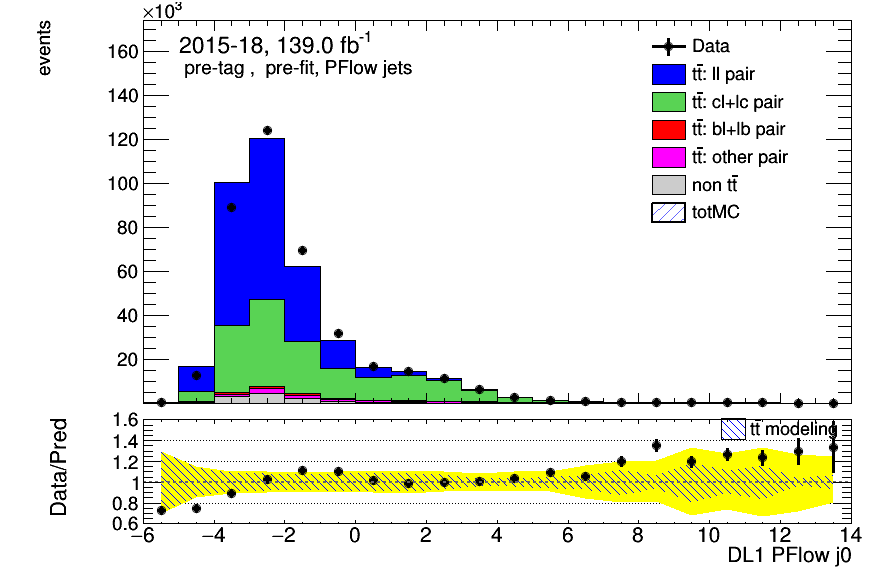
\includegraphics[width=1\textwidth]{Oct_distributions/pretagNoRwDL1rwithhighpTPFlow_scaledall/DataMC__J0_DL1.png}
\end{minipage}\hfill
\begin{minipage}[b]{.45\textwidth}
\centering
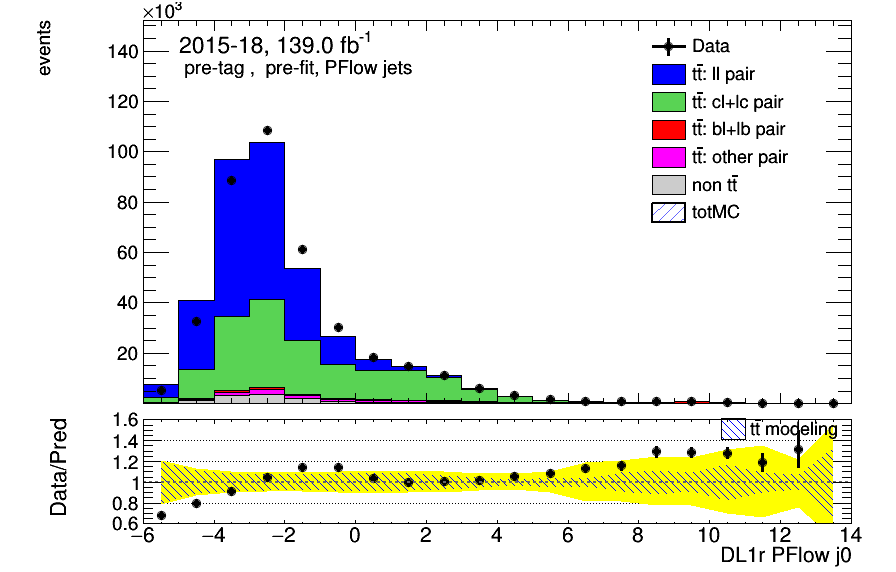
\includegraphics[width=1\textwidth]{Oct_distributions/pretagNoRwDL1rwithhighpTPFlow_scaledall/DataMC__J0_DL1r.png}
\end{minipage}\hfill
\begin{minipage}[b]{.45\textwidth}
\centering
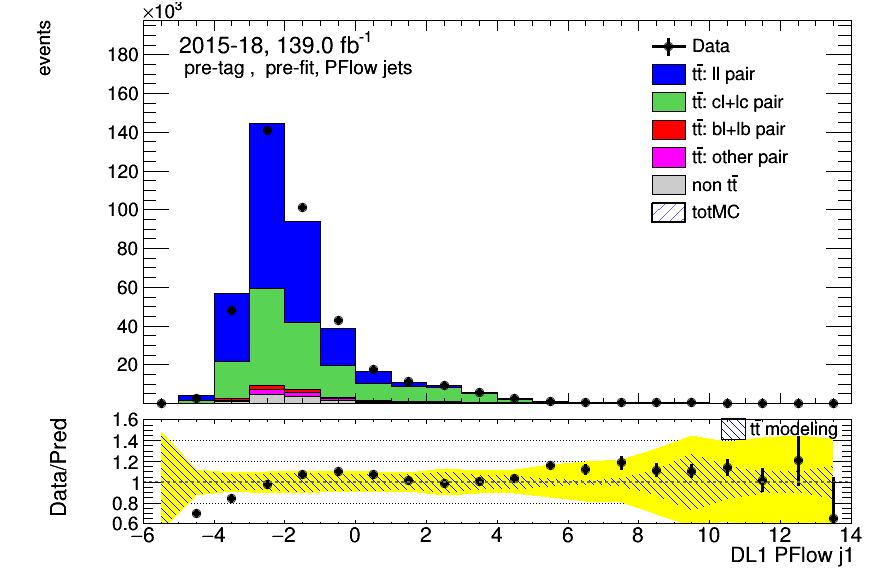
\includegraphics[width=1\textwidth]{Oct_distributions/pretagNoRwDL1rwithhighpTPFlow_scaledall/DataMC__J1_DL1.png}
\end{minipage}\hfill
\begin{minipage}[b]{.45\textwidth}
\centering
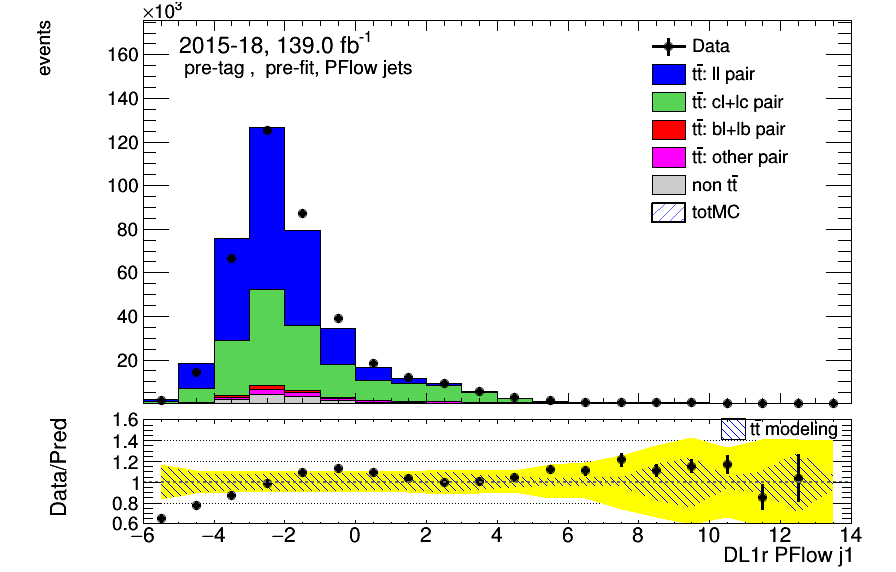
\includegraphics[width=1\textwidth]{Oct_distributions/pretagNoRwDL1rwithhighpTPFlow_scaledall/DataMC__J1_DL1r.png}
\end{minipage}\hfill
\begin{minipage}[b]{.45\textwidth}
\centering
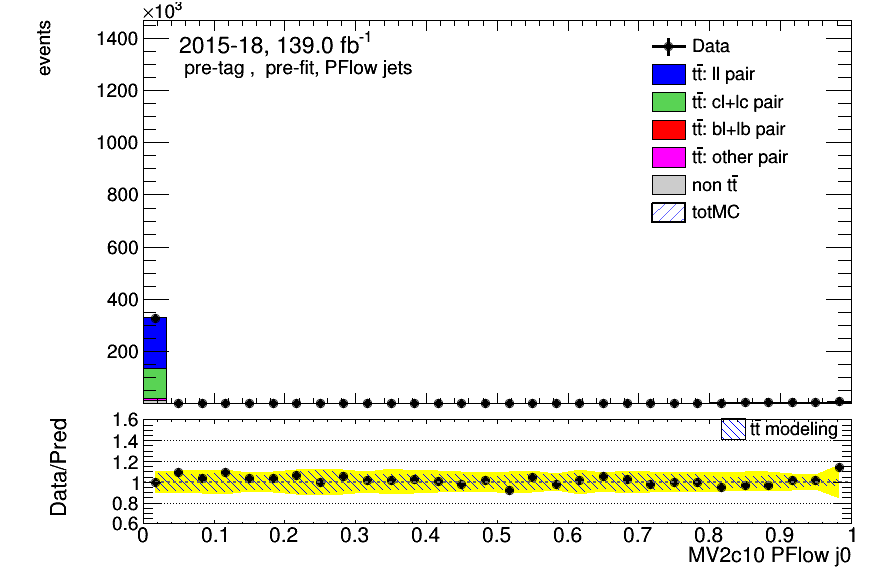
\includegraphics[width=1\textwidth]{Oct_distributions/pretagNoRwDL1rwithhighpTPFlow_scaledall/DataMC_J0_MV2c10.png}
\end{minipage}\hfill
\begin{minipage}[b]{.45\textwidth}
\centering
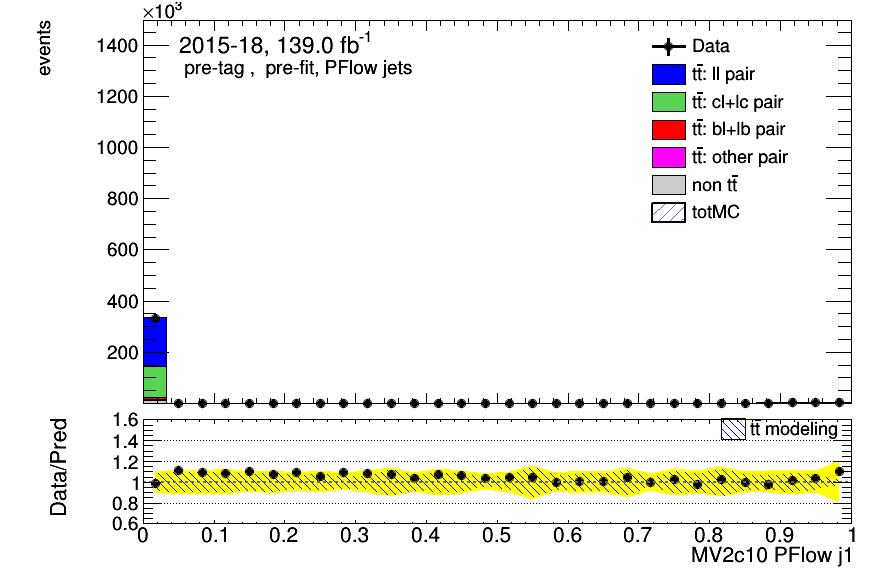
\includegraphics[width=1\textwidth]{Oct_distributions/pretagNoRwDL1rwithhighpTPFlow_scaledall/DataMC_J1_MV2c10.png}
\end{minipage}
\caption{Distributions of the DL1, DL1r and MV2c10 taggers output of the combination of the standard selection and the high-$p_T$ selection, before fitting or tagging with full uncertainties.} \label{fig:taggers_PFlow}
\end{figure}


\begin{figure}
\begin{minipage}[b]{.45\textwidth}
\centering
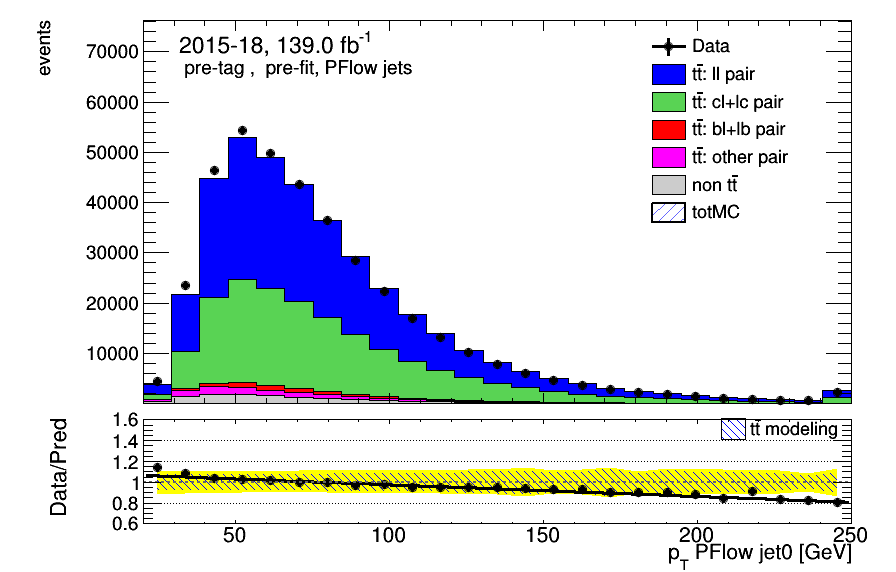
\includegraphics[width=1\textwidth]{Oct_distributions/pretagNoRwDL1rwithhighpTPFlow_scaledall/DataMC_J0_pt.png}
\end{minipage}\hfill
\begin{minipage}[b]{.45\textwidth}
\centering
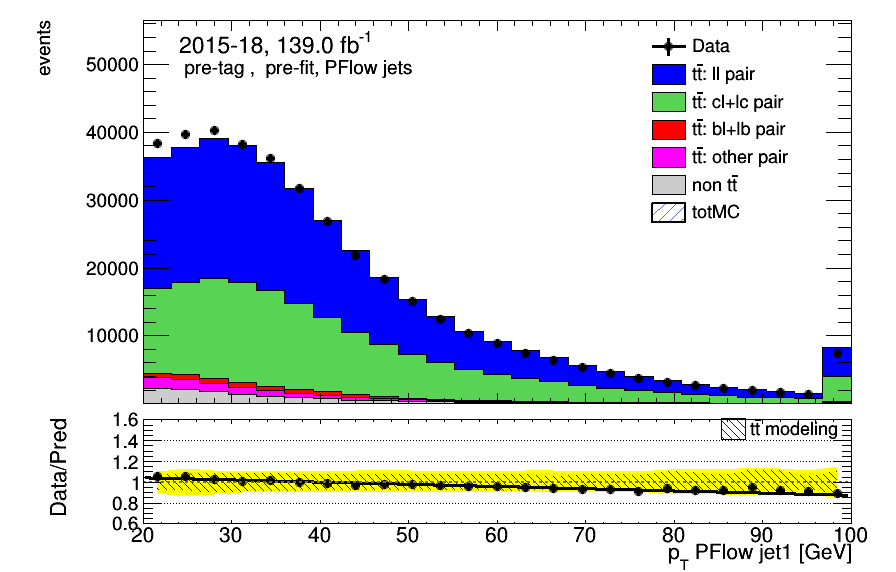
\includegraphics[width=1\textwidth]{Oct_distributions/pretagNoRwDL1rwithhighpTPFlow_scaledall/DataMC_J1_pt.png}
\end{minipage}\hfill
\begin{minipage}[b]{.45\textwidth}
\centering
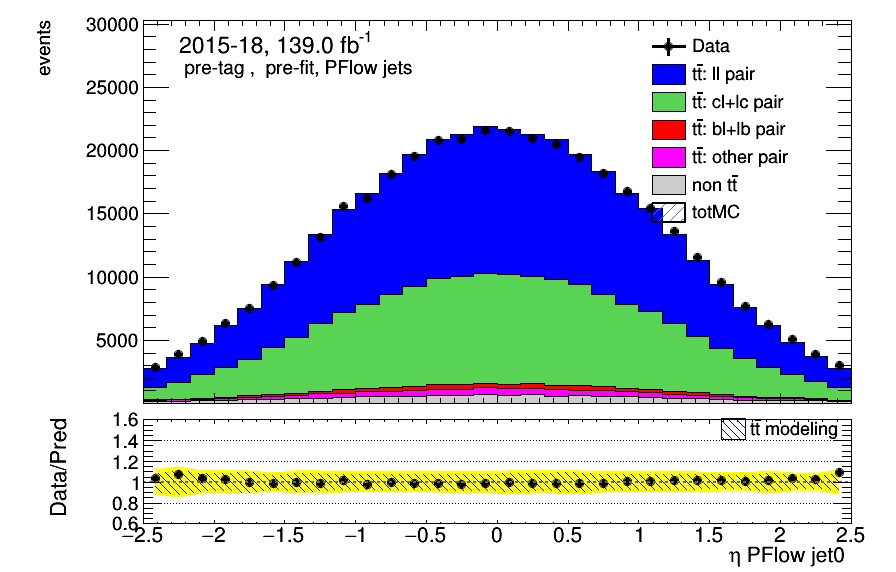
\includegraphics[width=1\textwidth]{Oct_distributions/pretagNoRwDL1rwithhighpTPFlow_scaledall/DataMC_J0_eta.png}
\end{minipage}\hfill
\begin{minipage}[b]{.45\textwidth}
\centering
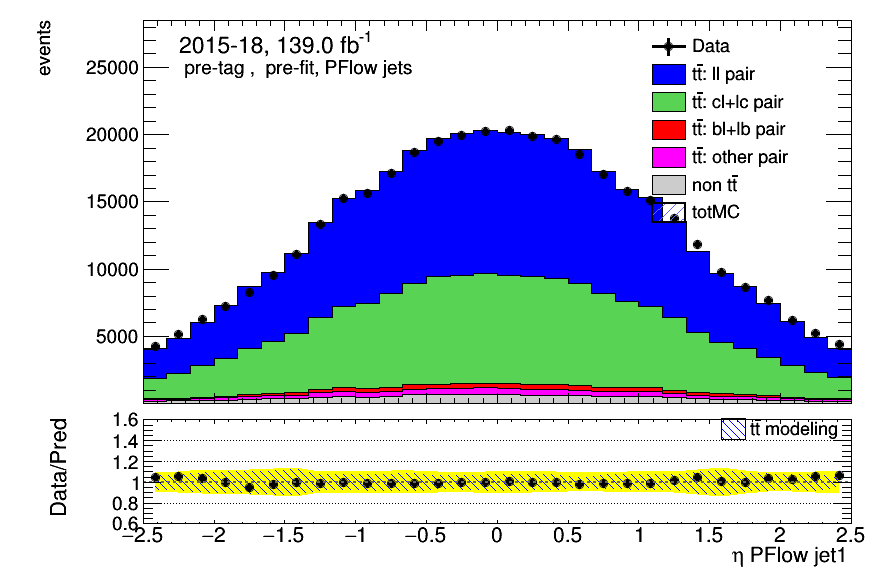
\includegraphics[width=1\textwidth]{Oct_distributions/pretagNoRwDL1rwithhighpTPFlow_scaledall/DataMC_J1_eta.png}
\end{minipage}\hfill
\begin{minipage}[b]{.45\textwidth}
\centering
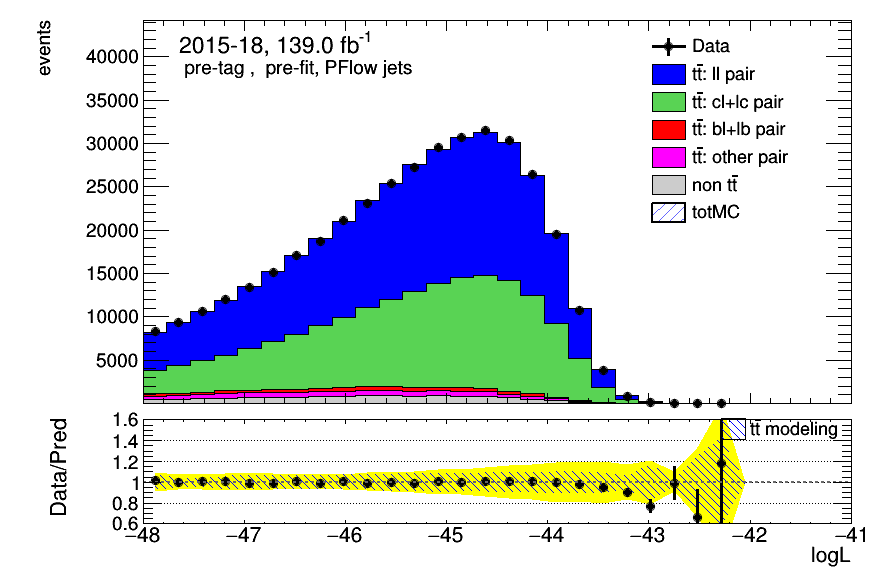
\includegraphics[width=1\textwidth]{Oct_distributions/pretagNoRwDL1rwithhighpTPFlow_scaledall/DataMC_LLR.png}
\end{minipage}\hfill
\begin{minipage}[b]{.45\textwidth}
\centering
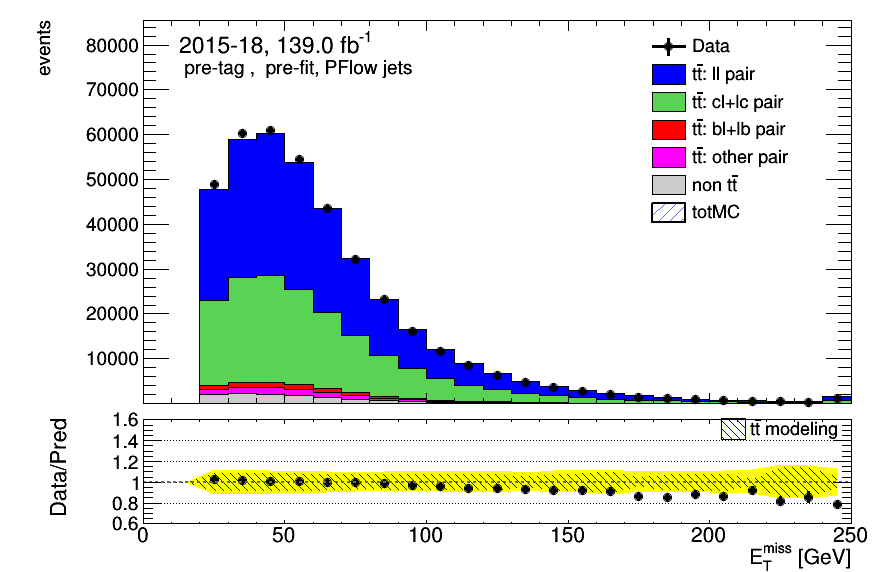
\includegraphics[width=1\textwidth]{Oct_distributions/pretagNoRwDL1rwithhighpTPFlow_scaledall/DataMC_MET.png}
\end{minipage}
\caption{Distributions of the leading and sub-leading jets from W decay, KLFitter output and the transverse missing transverse energy of the combination of the standard selection and the high-$p_T$ selection, before fitting or tagging with full uncertainties.} \label{fig:jets_PFlow}
\end{figure}




\begin{figure}
\begin{minipage}[b]{.45\textwidth}
\centering
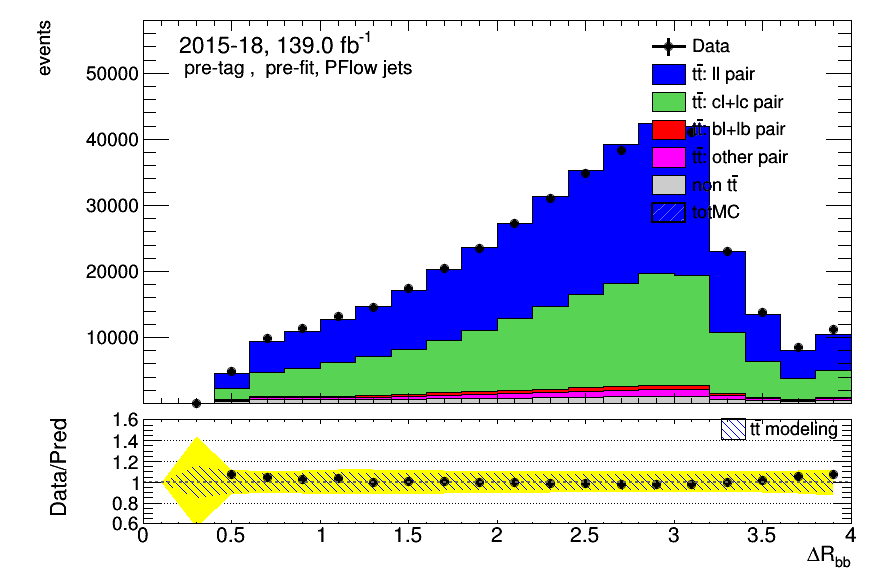
\includegraphics[width=1\textwidth]{Oct_distributions/pretagNoRwDL1rwithhighpTPFlow_scaledall/DataMC_dRbb.png}
\end{minipage}\hfill
\begin{minipage}[b]{.45\textwidth}
\centering
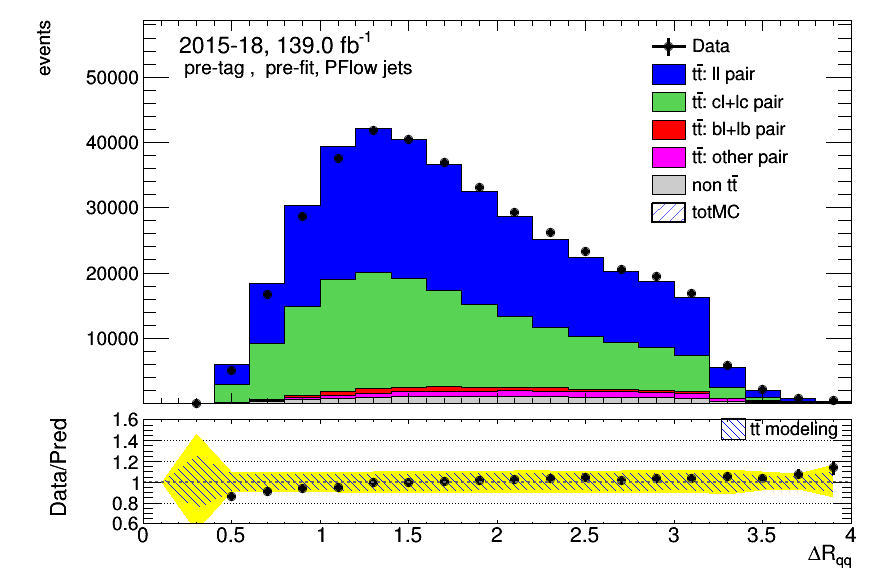
\includegraphics[width=1\textwidth]{Oct_distributions/pretagNoRwDL1rwithhighpTPFlow_scaledall/DataMC_dRqq.png}
\end{minipage}\hfill
\begin{minipage}[b]{.45\textwidth}
\centering
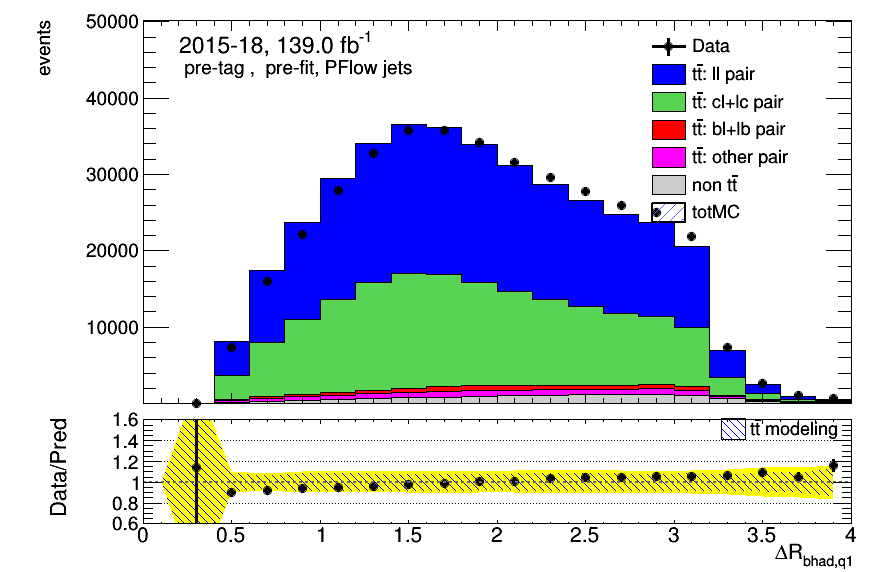
\includegraphics[width=1\textwidth]{Oct_distributions/pretagNoRwDL1rwithhighpTPFlow_scaledall/DataMC_dRbhadq1.png}
\end{minipage}\hfill
\begin{minipage}[b]{.45\textwidth}
\centering
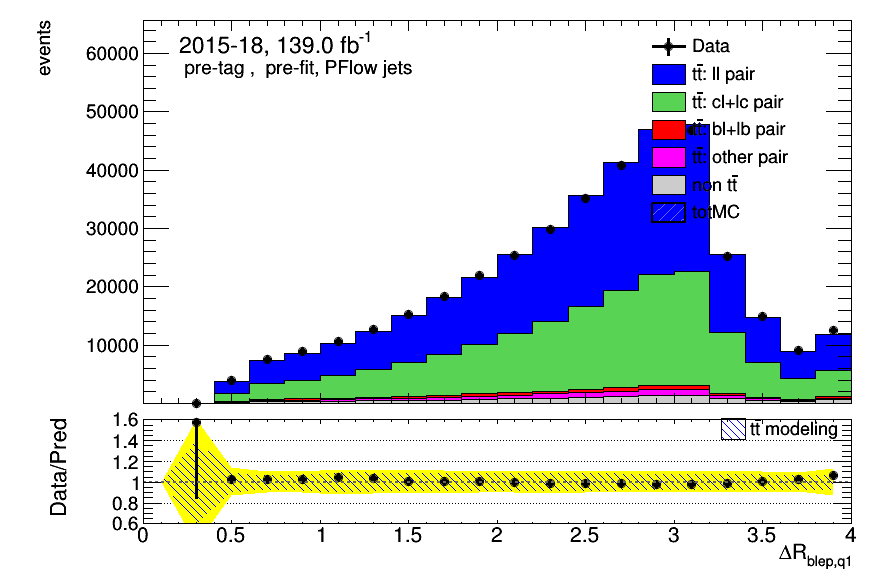
\includegraphics[width=1\textwidth]{Oct_distributions/pretagNoRwDL1rwithhighpTPFlow_scaledall/DataMC_dRblepq1.png} 
\end{minipage}\hfill
\begin{minipage}[b]{.45\textwidth}
\centering
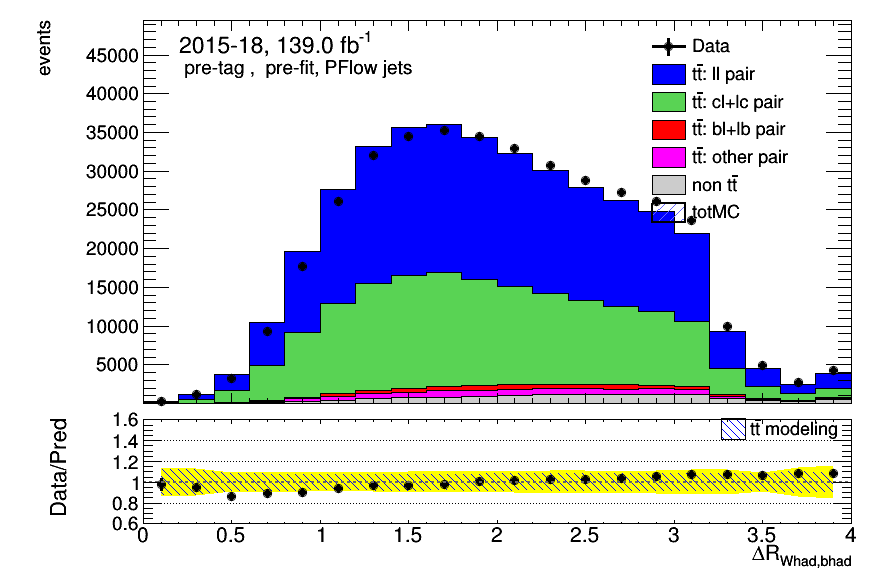
\includegraphics[width=1\textwidth]{Oct_distributions/pretagNoRwDL1rwithhighpTPFlow_scaledall/DataMC_dRWhadbhad.png} 
\end{minipage}\hfill
\begin{minipage}[b]{.45\textwidth}
\centering
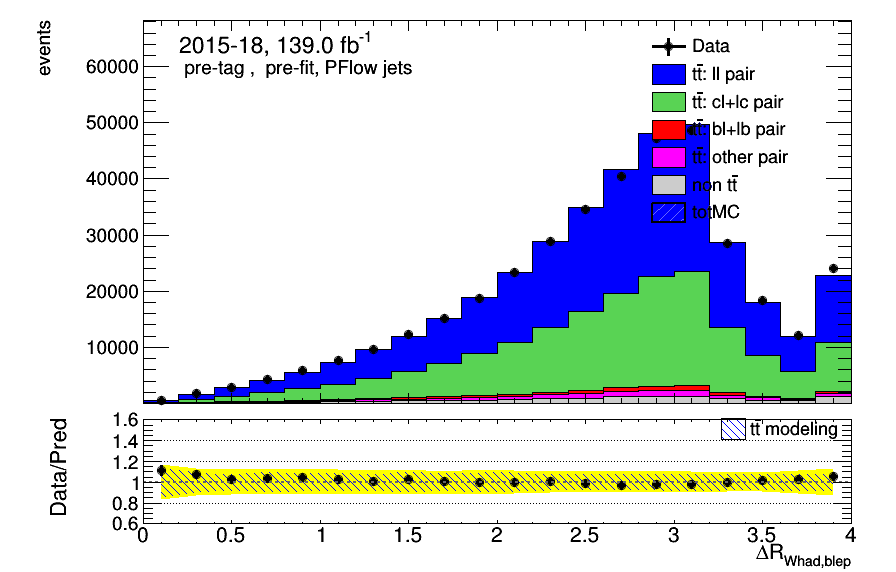
\includegraphics[width=1\textwidth]{Oct_distributions/pretagNoRwDL1rwithhighpTPFlow_scaledall/DataMC_dRWhadblep.png} 
\end{minipage}
\caption{Distributions of angle related variables of the combination of the standard selection and the high-$p_T$ selection, before fitting or tagging with full uncertainties.} \label{fig:angles_PFlow}
\end{figure}


\begin{figure}
\begin{minipage}[b]{.45\textwidth}
\centering
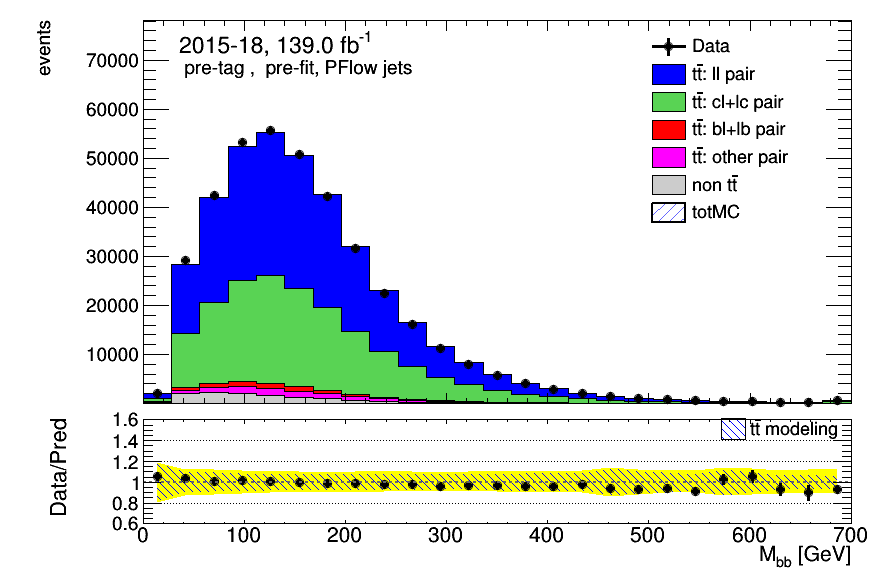
\includegraphics[width=1\textwidth]{Oct_distributions/pretagNoRwDL1rwithhighpTPFlow_scaledall/DataMC_Mbb.png}
\end{minipage}\hfill
\begin{minipage}[b]{.45\textwidth}
\centering
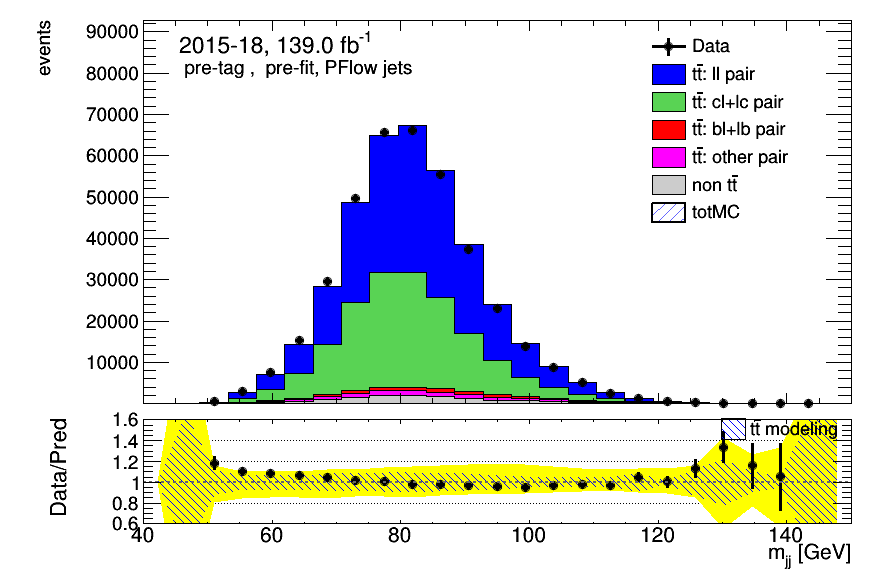
\includegraphics[width=1\textwidth]{Oct_distributions/pretagNoRwDL1rwithhighpTPFlow_scaledall/DataMC_mjj.png}
\end{minipage}
\begin{minipage}[b]{.45\textwidth}
\centering
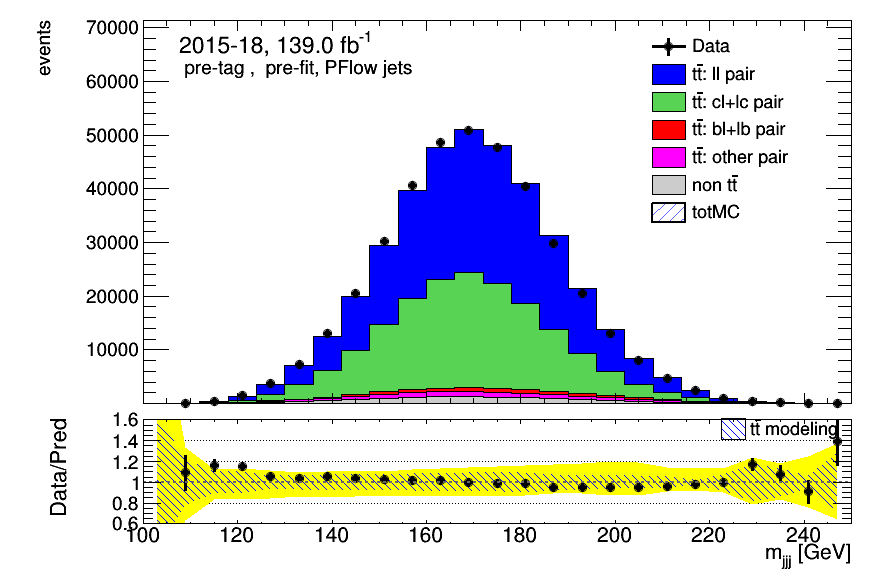
\includegraphics[width=1\textwidth]{Oct_distributions/pretagNoRwDL1rwithhighpTPFlow_scaledall/DataMC_mjjj.png}
\end{minipage}\hfill
\begin{minipage}[b]{.45\textwidth}
\centering
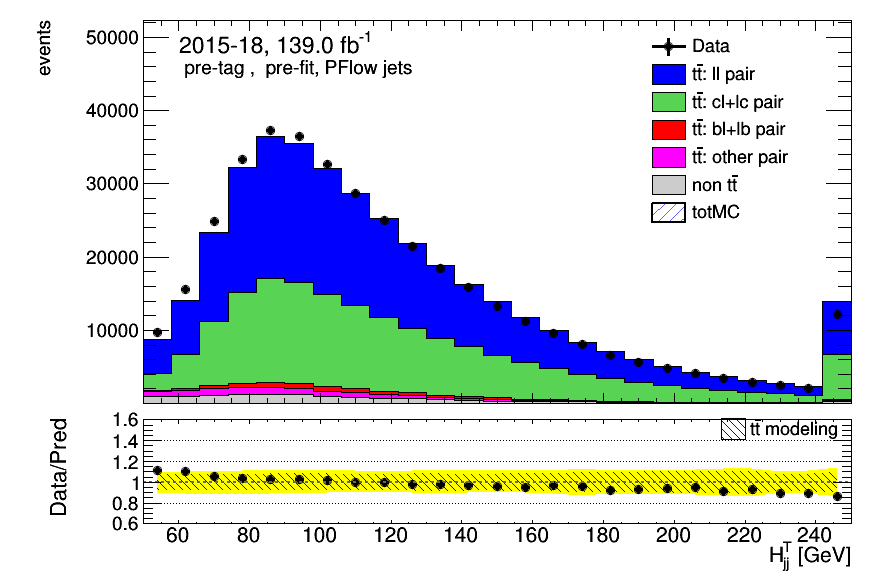
\includegraphics[width=1\textwidth]{Oct_distributions/pretagNoRwDL1rwithhighpTPFlow_scaledall/DataMC_Htjj.png}
\end{minipage}\hfill
\caption{Distributions of mass related variables of the combination of the standard selection and the high-$p_T$ selection, before fitting or tagging with stat-only uncertainties.} \label{fig:mass_PFlow}
\end{figure}

\newpage
\begin{figure}[h]
\begin{minipage}[b]{.45\textwidth}
\centering
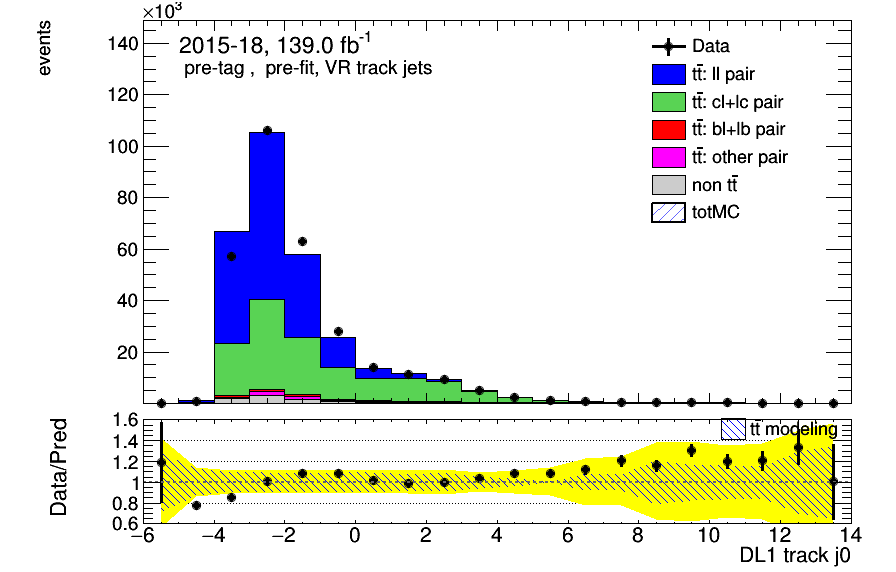
\includegraphics[width=1\textwidth]{Oct_distributions/pretagNoRwDL1rwithhighpTVRJets_scaledall/DataMC__J0_DL1.png}
\end{minipage}\hfill
\begin{minipage}[b]{.45\textwidth}
\centering
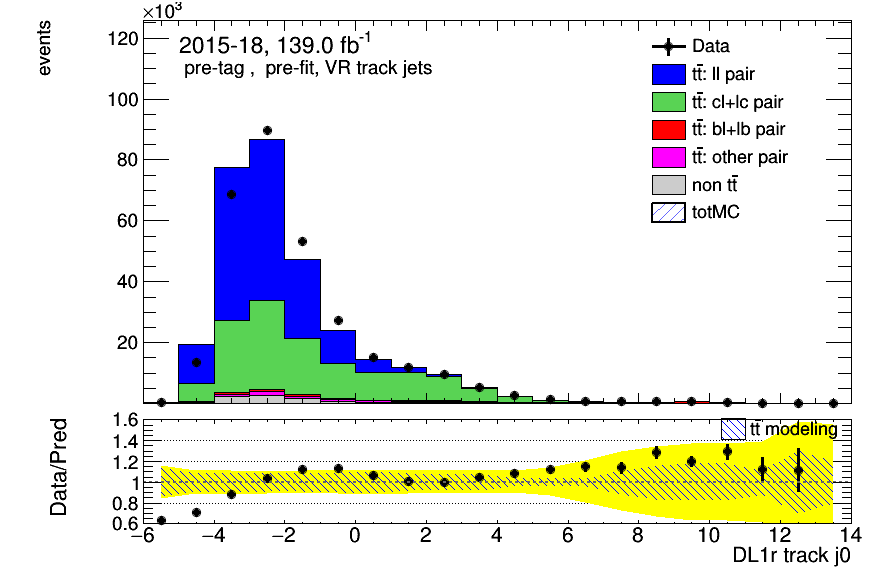
\includegraphics[width=1\textwidth]{Oct_distributions/pretagNoRwDL1rwithhighpTVRJets_scaledall/DataMC__J0_DL1r.png}
\end{minipage}\hfill
\begin{minipage}[b]{.45\textwidth}
\centering
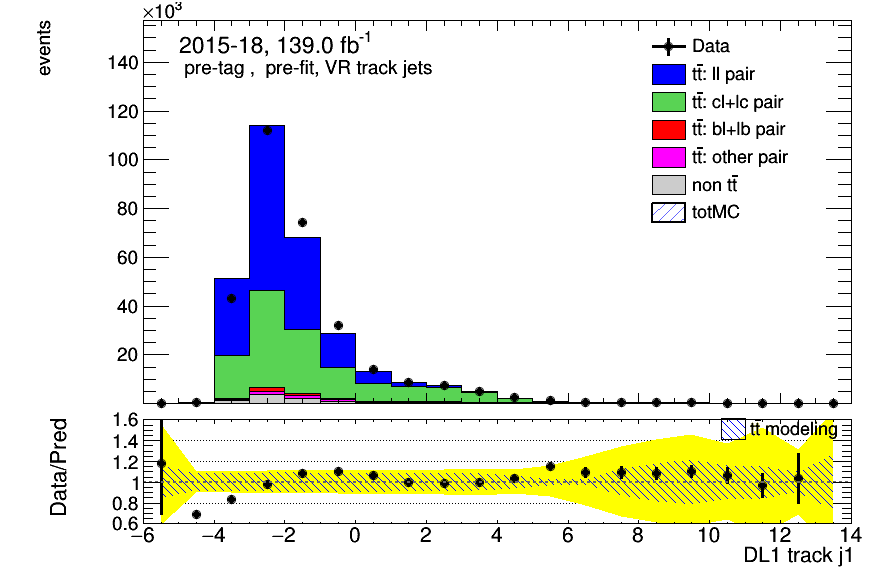
\includegraphics[width=1\textwidth]{Oct_distributions/pretagNoRwDL1rwithhighpTVRJets_scaledall/DataMC__J1_DL1.png}
\end{minipage}\hfill
\begin{minipage}[b]{.45\textwidth}
\centering
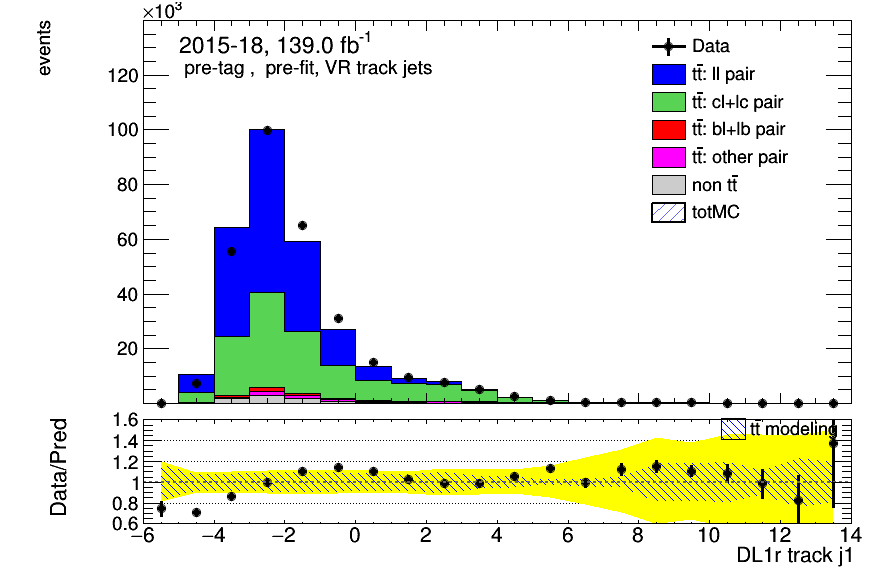
\includegraphics[width=1\textwidth]{Oct_distributions/pretagNoRwDL1rwithhighpTVRJets_scaledall/DataMC__J1_DL1r.png}
\end{minipage}\hfill
\begin{minipage}[b]{.45\textwidth}
\centering
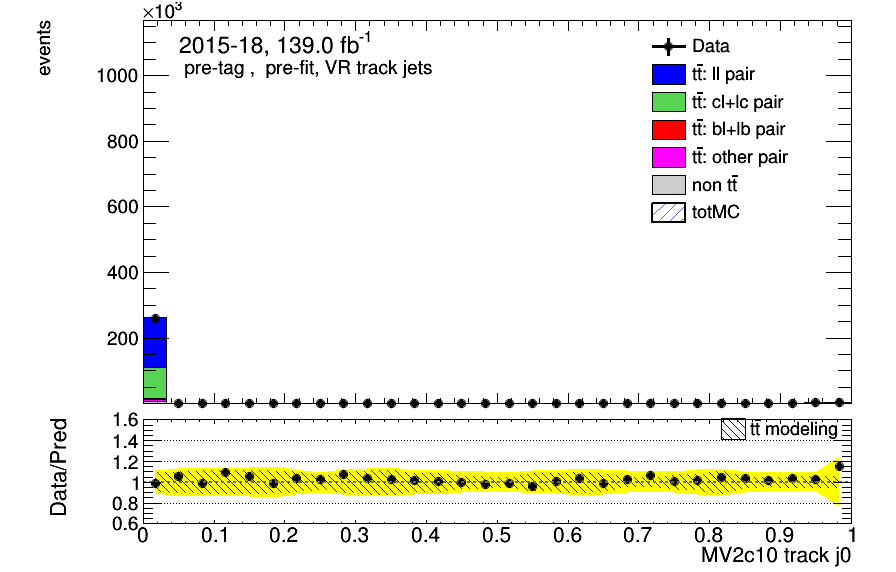
\includegraphics[width=1\textwidth]{Oct_distributions/pretagNoRwDL1rwithhighpTVRJets_scaledall/DataMC_J0_MV2c10.png}
\end{minipage}\hfill
\begin{minipage}[b]{.45\textwidth}
\centering
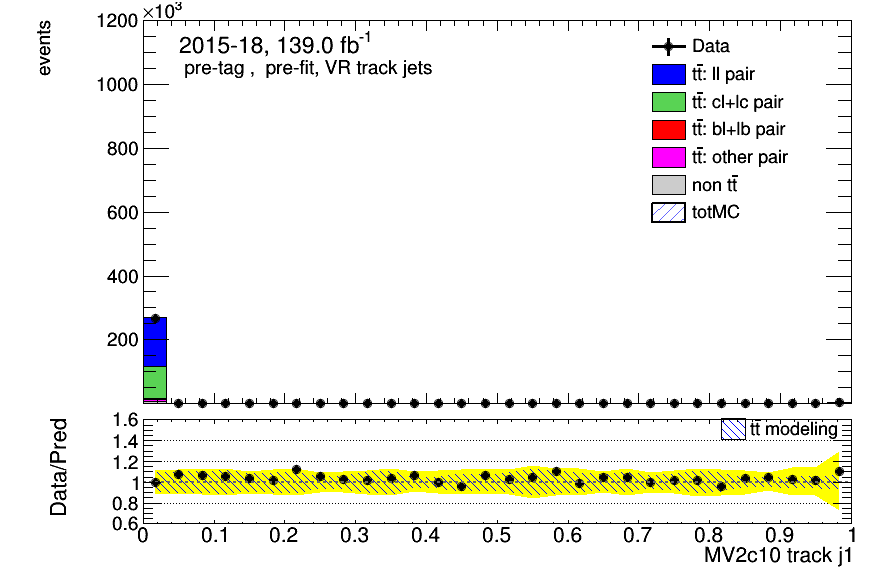
\includegraphics[width=1\textwidth]{Oct_distributions/pretagNoRwDL1rwithhighpTVRJets_scaledall/DataMC_J1_MV2c10.png}
\end{minipage}
\caption{Distributions of the DL1, DL1r and MV2c10 taggers output of the combination of the standard selection and the high-$p_T$ selection, before fitting or tagging with full uncertainties.} \label{fig:taggers_VRJets}
\end{figure}


\begin{figure}
\begin{minipage}[b]{.45\textwidth}
\centering
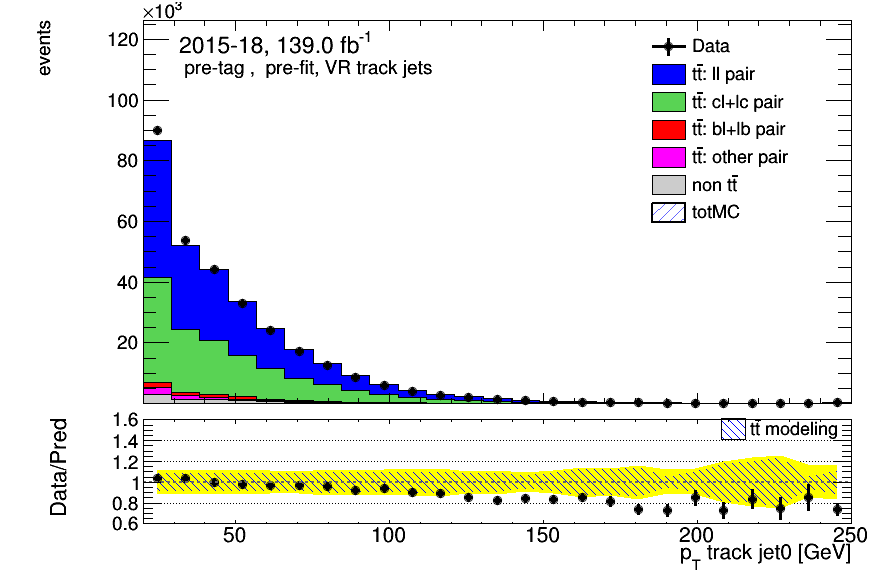
\includegraphics[width=1\textwidth]{Oct_distributions/pretagNoRwDL1rwithhighpTVRJets_scaledall/DataMC_J0_pt.png}
\end{minipage}\hfill
\begin{minipage}[b]{.45\textwidth}
\centering
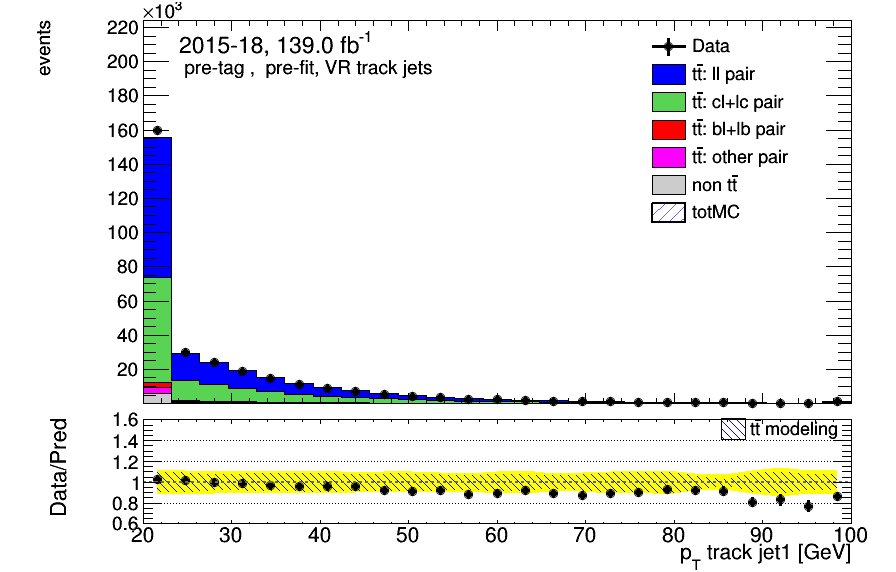
\includegraphics[width=1\textwidth]{Oct_distributions/pretagNoRwDL1rwithhighpTVRJets_scaledall/DataMC_J1_pt.png}
\end{minipage}\hfill
\begin{minipage}[b]{.45\textwidth}
\centering
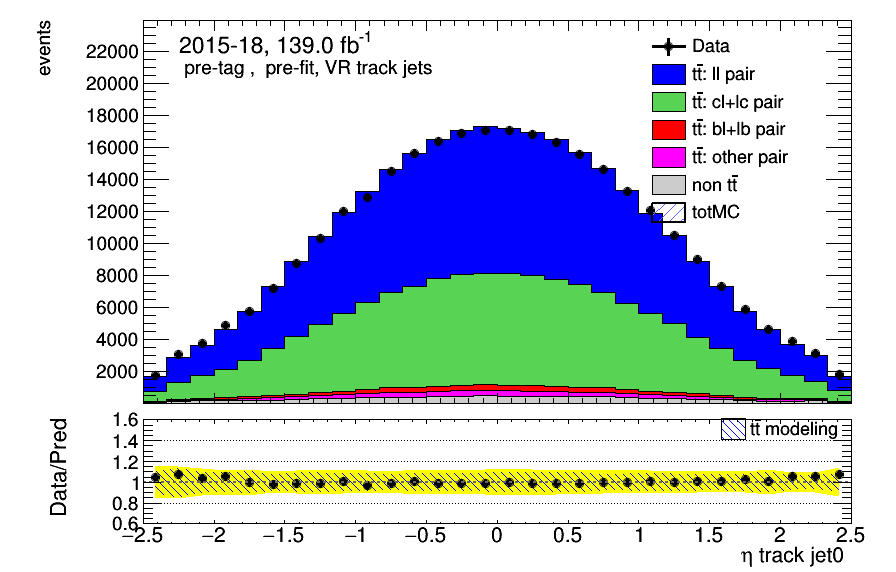
\includegraphics[width=1\textwidth]{Oct_distributions/pretagNoRwDL1rwithhighpTVRJets_scaledall/DataMC_J0_eta.png}
\end{minipage}\hfill
\begin{minipage}[b]{.45\textwidth}
\centering
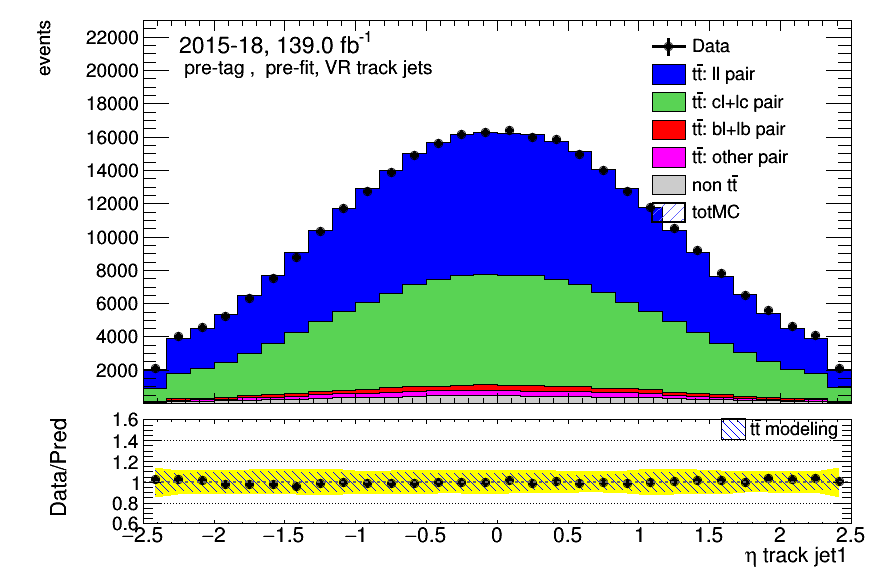
\includegraphics[width=1\textwidth]{Oct_distributions/pretagNoRwDL1rwithhighpTVRJets_scaledall/DataMC_J1_eta.png}
\end{minipage}\hfill
\begin{minipage}[b]{.45\textwidth}
\centering
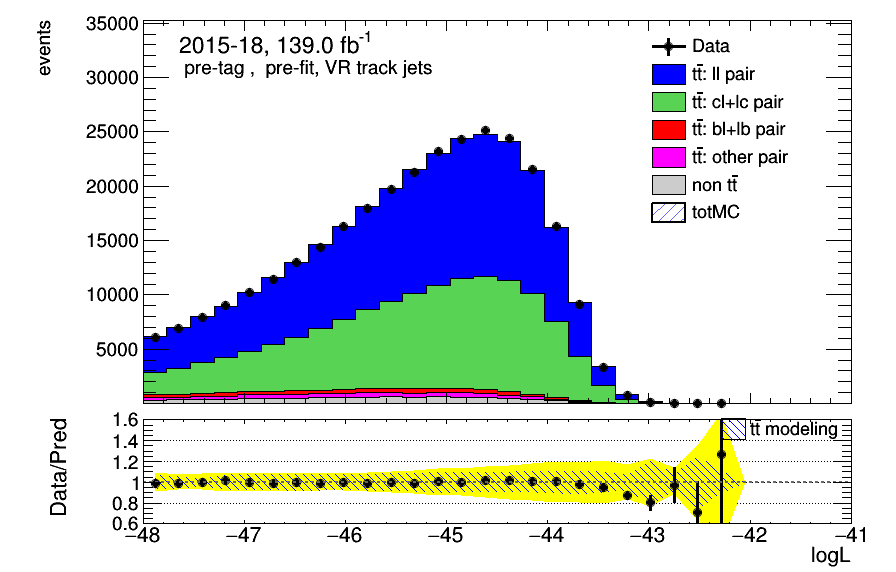
\includegraphics[width=1\textwidth]{Oct_distributions/pretagNoRwDL1rwithhighpTVRJets_scaledall/DataMC_LLR.png}
\end{minipage}\hfill
\begin{minipage}[b]{.45\textwidth}
\centering
\includegraphics[width=1\textwidth]{Oct_distributions/pretagNoRwDL1rwithhighpTVRJets_scaledall/DataMC_MET.png}
\end{minipage}
\caption{Distributions of the leading and sub-leading jets from W decay, KLFitter output and the transverse missing transverse energy of the combination of the standard selection and the high-$p_T$ selection, before fitting or tagging with full uncertainties.} \label{fig:jets_VRJets}
\end{figure}




\begin{figure}
\begin{minipage}[b]{.45\textwidth}
\centering
\includegraphics[width=1\textwidth]{Oct_distributions/pretagNoRwDL1rwithhighpTVRJets_scaledall/DataMC_dRbb.png}
\end{minipage}\hfill
\begin{minipage}[b]{.45\textwidth}
\centering
\includegraphics[width=1\textwidth]{Oct_distributions/pretagNoRwDL1rwithhighpTVRJets_scaledall/DataMC_dRqq.png}
\end{minipage}\hfill
\begin{minipage}[b]{.45\textwidth}
\centering
\includegraphics[width=1\textwidth]{Oct_distributions/pretagNoRwDL1rwithhighpTVRJets_scaledall/DataMC_dRbhadq1.png}
\end{minipage}\hfill
\begin{minipage}[b]{.45\textwidth}
\centering
\includegraphics[width=1\textwidth]{Oct_distributions/pretagNoRwDL1rwithhighpTVRJets_scaledall/DataMC_dRblepq1.png} 
\end{minipage}\hfill
\begin{minipage}[b]{.45\textwidth}
\centering
\includegraphics[width=1\textwidth]{Oct_distributions/pretagNoRwDL1rwithhighpTVRJets_scaledall/DataMC_dRWhadbhad.png} 
\end{minipage}\hfill
\begin{minipage}[b]{.45\textwidth}
\centering
\includegraphics[width=1\textwidth]{Oct_distributions/pretagNoRwDL1rwithhighpTVRJets_scaledall/DataMC_dRWhadblep.png} 
\end{minipage}
\caption{Distributions of angle related variables of the combination of the standard selection and the high-$p_T$ selection, before fitting or tagging with full uncertainties.} \label{fig:angles_VRJets}
\end{figure}


\begin{figure}
\begin{minipage}[b]{.45\textwidth}
\centering
\includegraphics[width=1\textwidth]{Oct_distributions/pretagNoRwDL1rwithhighpTVRJets_scaledall/DataMC_Mbb.png}
\end{minipage}\hfill
\begin{minipage}[b]{.45\textwidth}
\centering
\includegraphics[width=1\textwidth]{Oct_distributions/pretagNoRwDL1rwithhighpTVRJets_scaledall/DataMC_mjj.png}
\end{minipage}
\begin{minipage}[b]{.45\textwidth}
\centering
\includegraphics[width=1\textwidth]{Oct_distributions/pretagNoRwDL1rwithhighpTVRJets_scaledall/DataMC_mjjj.png}
\end{minipage}\hfill
\begin{minipage}[b]{.45\textwidth}
\centering
\includegraphics[width=1\textwidth]{Oct_distributions/pretagNoRwDL1rwithhighpTVRJets_scaledall/DataMC_Htjj.png}
\end{minipage}
\caption{Distributions of mass related variables of the combination of the standard selection and the high-$p_T$ selection, before fitting or tagging with stat-only uncertainties.} \label{fig:mass_VRJets}
\end{figure}

\subsubsection{Efficiencies and Scale Factors}

%The Monte Carlo simulation demonstrates good agreement in different kinematic variables with data. 
The Dl1 and DL1r $c$-jet efficiencies and scale factors with systematics uncertainties are calculated with 4 different fixed cut working points: 60\%, 70\%, 77\%, and 85\%, for the p4060 derivation, in December 2020. The results are shown in Figure \ref{fig:Dec_eff_PFlow}, \ref{fig:Dec_eff_VRJets}, \ref{fig:Dec_SF_PFlow}, \ref{fig:Dec_SF_VRJets}, for the charm jets mistagging efficiency and scale factors for the PFlow jet collections and the VR Track jets collections. These results combine the standard selection and the high $p_T$ selection, and a 1.25 $\pm$ 0.25 scale factor is applied on events with 3 true $b$ jets. The $c$-jets efficiencies and the scale factors are similar between the DL1 and DL1r as expected. 

% of the combination of the standard and the high-$p_T$ selection are calculated using the p3970 derivation with stat-only uncertainties, as shown in Figure \ref{fig:March_highpT_eff}, \ref{fig:March_highpT}. This result was not included in the official release due to time constraints, however, it will be included in the next round of calibration. The $c$-jet efficiencies and the scale factors are shown in the following: The calibration results of December 2019 are shown in the similar manner in the appendix, Figure \ref{fig:Dec}

%As the recommended tagger and jet collection is now DL1r and EMPFlow jet, in this report only r
 % are shown Fig\ref{fig:March_eff}, \ref{fig:March}. The efficiencies and scale factors
 % Results of the lastest calibration, March 2020 of p3970 in the form of DL1

% Efficiencies plots 

\begin{figure}[H]
\begin{minipage}[b]{.45\textwidth}
\centering
\includegraphics[width=1\textwidth]{SFplots_december/DL1allPFlowDec_DL1rallPFlowDec/eff60.png}
\end{minipage}\hfill
\begin{minipage}[b]{.45\textwidth}
\centering
\includegraphics[width=1\textwidth]{SFplots_december/DL1allPFlowDec_DL1rallPFlowDec/eff70.png}
\end{minipage}\hfill
\begin{minipage}[b]{.45\textwidth}
\centering
\includegraphics[width=1\textwidth]{SFplots_december/DL1allPFlowDec_DL1rallPFlowDec/eff77.png}
\end{minipage}\hfill
\begin{minipage}[b]{.45\textwidth}
\centering
\includegraphics[width=1\textwidth]{SFplots_december/DL1allPFlowDec_DL1rallPFlowDec/eff85.png}
\end{minipage}
\caption{Charm-jet efficiencies of PFlow jets collection of derivation p4060 in December 2020, given for 4 different working points.} \label{fig:Dec_eff_PFlow}
\end{figure}

\begin{figure}[H]
\begin{minipage}[b]{.45\textwidth}
\centering
\includegraphics[width=1\textwidth]{SFplots_december/DL1allVRJetsDec_DL1rallVRJetsDec/eff60.png}
\end{minipage}\hfill
\begin{minipage}[b]{.45\textwidth}
\centering
\includegraphics[width=1\textwidth]{SFplots_december/DL1allVRJetsDec_DL1rallVRJetsDec/eff70.png}
\end{minipage}\hfill
\begin{minipage}[b]{.45\textwidth}
\centering
\includegraphics[width=1\textwidth]{SFplots_december/DL1allVRJetsDec_DL1rallVRJetsDec/eff77.png}
\end{minipage}\hfill
\begin{minipage}[b]{.45\textwidth}
\centering
\includegraphics[width=1\textwidth]{SFplots_december/DL1allVRJetsDec_DL1rallVRJetsDec/eff85.png}
\end{minipage}
\caption{Charm-jet efficiencies of VR-Track jets collection of derivation p4060 in December 2020, given for 4 different working points.} \label{fig:Dec_eff_VRJets}
\end{figure}

% SF plots

\begin{figure}[H]
\begin{minipage}[b]{.45\textwidth}
\centering
\includegraphics[width=1\textwidth]{SFplots_december/DL1allPFlowDec_DL1rallPFlowDec/SF60.png}
\end{minipage}\hfill
\begin{minipage}[b]{.45\textwidth}
\centering
\includegraphics[width=1\textwidth]{SFplots_december/DL1allPFlowDec_DL1rallPFlowDec/SF70.png}
\end{minipage}\hfill
\begin{minipage}[b]{.45\textwidth}
\centering
\includegraphics[width=1\textwidth]{SFplots_december/DL1allPFlowDec_DL1rallPFlowDec/SF77.png}
\end{minipage}\hfill
\begin{minipage}[b]{.45\textwidth}
\centering
\includegraphics[width=1\textwidth]{SFplots_december/DL1allPFlowDec_DL1rallPFlowDec/SF85.png}
\end{minipage}
\caption{Charm-jet scale factors of PFlow jets collection of derivation p4060 in December 2020, given for 4 different working points.} \label{fig:Dec_SF_PFlow}
\end{figure}

\begin{figure}[H]
\begin{minipage}[b]{.45\textwidth}
\centering
\includegraphics[width=1\textwidth]{SFplots_december/DL1allVRJetsDec_DL1rallVRJetsDec/SF60.png}
\end{minipage}\hfill
\begin{minipage}[b]{.45\textwidth}
\centering
\includegraphics[width=1\textwidth]{SFplots_december/DL1allVRJetsDec_DL1rallVRJetsDec/SF70.png}
\end{minipage}\hfill
\begin{minipage}[b]{.45\textwidth}
\centering
\includegraphics[width=1\textwidth]{SFplots_december/DL1allVRJetsDec_DL1rallVRJetsDec/SF77.png}
\end{minipage}\hfill
\begin{minipage}[b]{.45\textwidth}
\centering
\includegraphics[width=1\textwidth]{SFplots_december/DL1allVRJetsDec_DL1rallVRJetsDec/SF85.png}
\end{minipage}
\caption{Charm-jet scale factors of VR-Track jets collection of derivation p4060 in December 2020, given for 4 different working points.} \label{fig:Dec_SF_VRJets}
\end{figure}


% maybe not neccessary to include the pseudocontinuous plots 

\iffalse
\begin{figure}[H]
\begin{minipage}[b]{.45\textwidth}
\centering
\includegraphics[width=1\textwidth]{SFplots_december/DL1allPFlowDec_DL1rallPFlowDec/SF60.png}
\end{minipage}\hfill
\begin{minipage}[b]{.45\textwidth}
\centering
\includegraphics[width=1\textwidth]{SFplots_december/DL1allPFlowDec_DL1rallPFlowDec/SF70.png}
\end{minipage}\hfill
\begin{minipage}[b]{.45\textwidth}
\centering
\includegraphics[width=1\textwidth]{SFplots_december/DL1allPFlowDec_DL1rallPFlowDec/SF77.png}
\end{minipage}\hfill
\begin{minipage}[b]{.45\textwidth}
\centering
\includegraphics[width=1\textwidth]{SFplots_december/DL1allPFlowDec_DL1rallPFlowDec/SF85.png}
\end{minipage}
\caption{Scale factors of calibration of derivation p3970 in March 2020, given for  4 different working points.} \label{fig:March}
\end{figure}



\begin{figure}[H]
\begin{minipage}[b]{.45\textwidth}
\centering
\includegraphics[width=1\textwidth]{March_highpT/eff60.png}
\end{minipage}\hfill
\begin{minipage}[b]{.45\textwidth}
\centering
\includegraphics[width=1\textwidth]{March_highpT/eff70.png}
\end{minipage}\hfill
\begin{minipage}[b]{.45\textwidth}
\centering
\includegraphics[width=1\textwidth]{March_highpT/eff77.png}
\end{minipage}\hfill
\begin{minipage}[b]{.45\textwidth}
\centering
\includegraphics[width=1\textwidth]{March_highpT/eff85.png}
\end{minipage}
\caption{Charm-jet efficiencies of calibration of derivation p3970 in March 2020, combining the standard and the high-$p_{T}$ selection, given for  4 different working points.} \label{fig:March_highpT_eff}
\end{figure}


\begin{figure}[H]
\begin{minipage}[b]{.45\textwidth}
\centering
\includegraphics[width=1\textwidth]{March_highpT/SF60.png}
\end{minipage}\hfill
\begin{minipage}[b]{.45\textwidth}
\centering
\includegraphics[width=1\textwidth]{March_highpT/SF70.png}
\end{minipage}\hfill
\begin{minipage}[b]{.45\textwidth}
\centering
\includegraphics[width=1\textwidth]{March_highpT/SF77.png}
\end{minipage}\hfill
\begin{minipage}[b]{.45\textwidth}
\centering
\includegraphics[width=1\textwidth]{March_highpT/SF85.png}
\end{minipage}
\caption{Scale factors of calibration of derivation p3970 in March 2020, combining the standard and the high-$p_{T}$ selection, given for  4 different working points.} \label{fig:March_highpT}
\end{figure}



In terms of statistical gain, taking the 60\% working point scale factor with 2018 data as an example, the error is reduced as expected. In the last bin of the $p_{T}$ distribution of scale factors, the error is reduced by 55\%, which suggests the success of high-$p_{T}$ selection method. The percentage reduction of error of each bin is given in Tab.\ref{tab:limit}:


 \begin{table}[h]
 \begin{centering}
 \begin{tabular}{|p{2.5em}||p{2.5em}|p{2.5em}|p{5em}||p{2.5em}|p{2.5em}|p{5em}||p{5em}|}
          \hline
          & \multicolumn{3}{|c||}{high-$p_{T}$ + standard selection} & \multicolumn{3}{|c||}{standard selection only} & \\  \hline\hline
          Bins& Bin Value &Bin error&Percentage error&Bin Value &Bin error&Percentage error & Error reduction\\ \hline
          Bin 1 & 1.25 & 0.12 & 10\% &1.20 & 0.13 & 11\% & 11\% \\ \hline
          Bin 2 & 1.34 & 0.10 & 8\% & 1.24 & 0.11 & 9\% & 18\% \\ \hline
          Bin 3 & 1.22 & 0.10 & 8\% & 1.04 & 0.11 & 10\% & 28\% \\ \hline
          Bin 4 & 0.98 & 0.24 & 24\% & 0.72 & 0.27 & 37\% & 55\% \\ \hline
          
 
 \end{tabular} 
 \caption{Bins values and the corresponding errors of the scale factor at 60\% working point, with 2018 data.}
 \end{centering}
 \label{tab:limit}
 \end{table}

\fi

\newpage
\printbibliography
% \begin{thebibliography}{99}

% \bibitem{HIGG-2018-04} ATLAS Collaboration,\textit{Observation of $H\rightarrow bb$ decays andV Hproduction with the ATLAS detector},Phys. Lett. B786(2018) 59, \href{http://arxiv.org/abs/1808.08238}{arXiv:1808.08238 [hep-ex]}.
% \bibitem{HIGG-2018-13} ATLAS Collaboration,\textit{Observation of Higgs boson production in association with a top quark pairat the LHC with the ATLAS detector}, Phys. Lett. B784(2018) 173, \href{http://arxiv.org/abs/1806.00425}{arXiv:1806.00425 [hep-ex]}.
% \bibitem{PERF-2012-04} ATLAS Collaboration, \textit{Performance of $b$-jet identification in the ATLAS experiment}, JINST11(2016) P04008, \href{http://arxiv.org/abs/1512.01094}{arXiv:1512.01094 [hep-ex]}.
% \bibitem{PERF-2016-05} ATLAS Collaboration,\textit{Measurements of $b$-jet tagging efficiency with the ATLAS detector using $t\bar{t}$ events at$\sqrt{s}$=13TeV}, JHEP08(2018) 089, \href{http://arxiv.org/abs/1805.01845}{arXiv:1805.01845 [hep-ex]}.
%  \bibitem{SUSY-2014-08} ATLAS Collaboration, \textit{Measurements of Higgs boson properties in the diphoton decay channel with 36 fb−1 of pp collision data at s√=13 TeV with the ATLAS detector}, CERN-PH-EP-2015-214, 2015, \small{arXiv:}\href{http://arxiv.org/abs/arXiv:1508.06608} {1508.06608}.\normalsize
%  \bibitem{FTAG-2018-01} ATLAS Collaboration, \textit{measurement with $t\bar{t}$ events in pp collisions at $\sqrt{s}$ =13 TeV}, Eur. Phys. J. C 79, 970 (2019), \href{https://arxiv.org/abs/1907.05120}{arXiv:1907.05120}. 
% \bibitem{ATLAS-CONF-2018-006} ATLAS Collaboration, \textit{Calibration of light-flavour b-jet mistagging rates using ATLAS proton-proton collision data at \sqrt{s}=13TeV}, ATLAS-CONF-2018-006, \href{https://cds.cern.ch/record/2314418}{url:https://cds.cern.ch/record/2314418}
%  \bibitem{ATLAS-CONF-2018-043h} \textit{Combination of searches for Higgs boson pairs in $p\bar{p}$ collisions at 13 TeV with the ATLAS experiment}, ATLAS-CONF-2018-043, 2018, \href{https://cds.cern.ch/record/2638212?ln=en}{https://cds.cern.ch/record/2638212?ln=en}
% \bibitem{Interpreting Higgs result}, Dean Carmi, et al., \textit{Interpreting LHC Higgs Results from Natural New Physics Perspective}, \href{https://arxiv.org/abs/1202.3144}{arXiv:1202.3144}[hep-ph]. 
% \bibitem{ATLAS-CONF-2018-045} ATLAS Collaboration,\textit{Calibration of the ATLASb-tagging algorithm int ̄tsemileptonic events},ATLAS-CONF-2018-045, 2018,\href{http://cds.cern.ch/record/2638455}{url:https://cds.cern.ch/record/2638455}
% \bibitem{ATLAS-CONF-2018-006}ATLAS Collaboration, \textit{Calibration of light-flavour $b$-jet mistagging rates using ATLAS proton-proton collision data at $\sqrt{s}=13$~TeV}, ATLAS-CONF-2018-006, \small{url:} \href{https://cds.cern.ch/record/2314418}{https://cds.cern.ch/record/2314418}\normalsize
% \bibitem{cjet} ATLAS Collaboration, \textit{Measurement of $c$-jet tagging efficiency in $t\bar{t}$ events using a likelihood approach}, Feb 2017, \small{CDS: }\href{https://cds.cern.ch/record/2243764?ln=en}{ATL-COM-PHYS-2017-073}.\normalsize
% \bibitem{PDG}M. Tanabashiet al.(Particle Data Group), \textit{Review of Particle Physics}, Phys. Rev. D98, 030001 (2018), \href{https://link.aps.org/doi/10.1103/PhysRevD.98.030001}{doi:10.1103/PhysRevD.98.030001}.
% \bibitem{tagging} ATLAS collaboration, \textit{B Tagging in ATLAS and CMS}, Sep 2017, \small{arXiv:}\href{https://arxiv.org/abs/1709.01290}{1709.01290}\normalsize
% \bibitem{ATL-PHYS-PUB-2017-013}ATLAS Collaboration, \textit{Optimisation and performance studies of the ATLAS b-tagging algorithms for the 2017-18 LHC run}, \small{CDS:}\href{https://cds.cern.ch/record/2273281}{ATL-PHYS-PUB-2017-013}\normalsize
% \bibitem{FTAG-2018-01}ATLAS Collaboration, \textit{ATLAS $b$-jet identification performance and efficiency measurement with $t\bar{t}$ events in $pp$ collisions at $\sqrt{s}=13$ TeV,} Jan 2020,\small{arXiv:}\href{https://arxiv.org/abs/1907.05120}{1907.05120}\normalsize
% \bibitem{ATL-PHYS-PUB-2017-003} ATLAS Collaboration, \textit{FTAG-2018-01 of Jets Containing b-Hadrons with Recurrent Neural Networks at the ATLAS Experiment,} Jul 2017,\small{CDS: }\href{https://cds.cern.ch/record/2255226/files/ATL-PHYS-PUB-2017-003.pdf}{ATL-PHYS-PUB-2017-003}.\normalsize



% \bibitem{CKM1}G. Abbiendi et al., \textit{A Measurement of the rate of charm production in $W$ decays}, 1022 Phys. Lett. B490 (2000) 71, \small{arXiv: }\href{https://arxiv.org/abs/hep-ex/0009020}{hep-ex/0009020}.\normalsize
% \bibitem{CKM2}K. A. Olive 1023 et al., \textit{Review of Particle Physics}, \href{https://iopscience.iop.org/article/10.1088/1674-1137/38/9/090001}{Chin. Phys. C38 (2014) 090001}.\normalsize
% \bibitem{ttbar+HF SF}ATLAS collaboration, \textit{Measurement of the Higgs boson decaying to $b$-quarks produced in association with a top-quark pair in $pp$ collisions at $\sqrt{s}$=13 TeV with the ATLAS detector}, \href{http://cdsweb.cern.ch/record/2743685/files/ATLAS-CONF-2020-058.pdf}{ATLAS-CONF-2020-058}.



% \bibitem{ERDMANN201418}J Erdmann et al., \textit{A likelihood-based reconstruction algorithm for top-quark pairs and the KLFitter framework,} \small{DOI: }\href{https://doi.org/10.1016/j.nima.2014.02.029}{10.1016}.\normalsize
% \bibitem{DAPR-2010-01}ATLAS Collaboration, \texit{Luminosity determination in \(pp\) collisions at \(\sqrt{s} = 7\,\text{TeV}\) using the ATLAS detector at the LHC}, Eur. Phys. J. C, 2011, DOI:\href{https://link.springer.com/article/10.1140/epjc/s10052-011-1630-5}{10.1140/epjc/s10052-011-1630-5}.
% \bibitem{DAPR-2011-01}ATLAS Collaboration, \texit{Improved luminosity determination in \(pp\) collisions at \(\sqrt{s} = 7\,\text{TeV}\) using the ATLAS detector at the LHC}, Eur. Phys. J. C, 2013, DOI:\href{https://link.springer.com/article/10.1140/epjc/s10052-011-1630-5}{10.1140/epjc/s10052-013-2518-3}. 
% \bibitem{DAPR-2013-01}ATLAS Collaboration, \texit{Luminosity determination in \(pp\) collisions at \(\sqrt{s} = 8\,\text{TeV}\) using the ATLAS detector at the LHC}, Eur. Phys. J. C, 2016, DOI:\href{https://dspace.ankara.edu.tr/xmlui/handle/20.500.12575/67072}{10.1140/epjc/s10052-016-4466-1}. 
% \bibitem{LUCID2} G. Avoni and others,\texit{The new LUCID-2 detector for luminosity measurement and monitoring in ATLAS}, JINST, 2018, doi:\href{https://iopscience.iop.org/article/10.1088/1748-0221/13/07/P07017}{10.1088/1748-0221/13/07/P07017}.
% \bibitem{Aad:2020uyd} ATLAS Collaboration, \texit{Performance of the ATLAS muon triggers in Run 2}, CERN-EP-2020-031, 2020, DOI:\href{http://eprints.gla.ac.uk/225988/}{10.1088/1748-0221/15/09/p09015}.
% \bibitem{TRIG-2018-05}ATLAS Collaboration, \texit{Performance of electron and photon triggers in ATLAS during LHC Run~2}, Eur. Phys. J. C, 2020, \href{https://link.springer.com/article/10.1140/epjc/s10052-019-7500-2}{DOI:10.1140/epjc/s10052-019-7500-2}.
% \bibitem{powheg}S. Alioli, P. Nason, C. Oleari and E. Re, \textit{A general framework for implementing NLO calculations in shower Monte Carlo programs: the POWHEG BOX}, JHEP 06 (2010) 043, \small{arXiv:} \href{https://arxiv.org/abs/1002.2581}{1002.2581 [hep-ph]}.\normalsize
% \bibitem{evtgen} D. J. Lange, \textit{The EvtGen particle decay simulation package}, \href{https://www.sciencedirect.com/science/article/pii/S0168900201000894?via\%3Dihub}{Nucl. Instrum. Meth. A 462 (2001) 152}.\normalsize
% \bibitem{pythia}T. Sjöstrand, S. Mrenna and P. Skands, \textit{PYTHIA 6.4 physics and manual}, JHEP 05 (2006) 026, \small{arXiv: }\href{https://arxiv.org/abs/hep-ph/0603175}{hep-ph/0603175}.\normalsize
% \bibitem{perugia}P. Skands, \textit{Tuning Monte Carlo generators: The Perugia tunes}, Phys. Rev. D 82 (2010) 074018, \small{arXiv: }\href{https://arxiv.org/abs/1005.3457}{1005.3457 [hep-ph]}.\normalsize
% \bibitem{NNLO}M. Czakon, M. L. Mangano, A. Mitov and J. Rojo, \textit{Constraints on the gluon PDF from top quark pair production at hadron colliders}, JHEP 07 (2013) 167, \small{arXiv:} \href{https://arxiv.org/abs/1303.7215}{1303.7215 [hep-ph]}.\normalsize
% \bibitem{sherpa}T. Gleisberg et al., \textit{Event generation with SHERPA 1.1}, JHEP 02 (2009) 007, \small{arXiv:} \href{https://arxiv.org/abs/0811.4622}{0811.4622 [hep-ph]}.\normalsize
% \bibitem{GEANT4}S. Agostinelli et al., \textit{GEANT4 - a simulation toolkit},\href{https://www.sciencedirect.com/science/article/pii/S0168900203013688?via\%3Dihub}{ Nucl. Instrum. Meth. A 506 (2003) 250}.\normalsize


% \bibitem{ATL-PHYS-PUB-2017-0132016}Optimisation of the ATLAS b-tagging performance for the 2016 LHC Run, (2016),url: https://cds.cern.ch/record/2160731.


% \end{thebibliography}
 
\newpage

\appendix
\subsection{Appendix}
\newpage
\newpage

\begin{figure}[h]
\begin{minipage}[b]{.45\textwidth}
\centering
\includegraphics[width=1\textwidth]{Distribution_March/DataMC_J0_DL1.png}
\end{minipage}\hfill
\begin{minipage}[b]{.45\textwidth}
\centering
\includegraphics[width=1\textwidth]{Distribution_March/DataMC_J0_DL1r.png}
\end{minipage}\hfill
\begin{minipage}[b]{.45\textwidth}
\centering
\includegraphics[width=1\textwidth]{Distribution_March/DataMC_J0_eta.png}
\end{minipage}\hfill
\begin{minipage}[b]{.45\textwidth}
\centering
\includegraphics[width=1\textwidth]{Distribution_March/DataMC_J0_pt.png}
\end{minipage}\hfill
% \begin{minipage}[b]{.45\textwidth}
% \centering
% \includegraphics[width=1\textwidth]{Distribution_March/DataMC_LLR.png}
% \end{minipage}\hfill
\begin{minipage}[b]{.45\textwidth}
\centering
\includegraphics[width=1\textwidth]{Distribution_March/DataMC_Mbb.png}
\end{minipage}\hfill
% \begin{minipage}[b]{.45\textwidth}
% \centering
% \includegraphics[width=1\textwidth]{Distribution_March/DataMC_MET.png}
% \end{minipage}\hfill
\begin{minipage}[b]{.45\textwidth}
\centering
\includegraphics[width=1\textwidth]{Distribution_March/DataMC_mjj.png}
\end{minipage}
% \begin{minipage}[b]{.45\textwidth}
% \centering
% \includegraphics[width=1\textwidth]{Distribution_March/DataMC_dRJJ.png}
% \end{minipage}\hfill
\caption{Standard selection: various kinematic distributions of the standard selection before fitting or tagging with systematics. The top two plots are the distributions of the DL1 and Dl1r score distributions of the leading jet.} \label{fig:standard_selection}
\end{figure}

\begin{figure}[H]
\begin{minipage}[b]{.45\textwidth}
\centering
\includegraphics[width=1\textwidth]{Distribution_March/DataMC_J1_DL1.png}
\end{minipage}\hfill
\begin{minipage}[b]{.45\textwidth}
\centering
\includegraphics[width=1\textwidth]{Distribution_March/DataMC_J1_DL1r.png}
\end{minipage}\hfill
\begin{minipage}[b]{.45\textwidth}
\centering
\includegraphics[width=1\textwidth]{Distribution_March/DataMC_J1_eta.png}
\end{minipage}\hfill
\begin{minipage}[b]{.45\textwidth}
\centering
\includegraphics[width=1\textwidth]{Distribution_March/DataMC_J1_pt.png}
\end{minipage}
\caption{Selection for low-$p_T$ extension: kinematic distributions of the sub-leading $W$ decay jet before fitting or tagging with systematics. The top two plots are distributions of the DL1 and Dl1r score of the sub-leading jet.} \label{fig:lowpT_selection}
\end{figure}


\begin{figure}[H]
\begin{minipage}[b]{.45\textwidth}
\centering
\includegraphics[width=1\textwidth]{Distribution_March_highpT/DataMC_J0_DL1.png}
\end{minipage}\hfill
\begin{minipage}[b]{.45\textwidth}
\centering
\includegraphics[width=1\textwidth]{Distribution_March_highpT/DataMC_J0_DL1r.png}
\end{minipage}\hfill
\begin{minipage}[b]{.45\textwidth}
\centering
\includegraphics[width=1\textwidth]{Distribution_March_highpT/DataMC_J0_eta.png}
\end{minipage}\hfill
\begin{minipage}[b]{.45\textwidth}
\centering
\includegraphics[width=1\textwidth]{Distribution_March_highpT/DataMC_J0_pt.png}
\end{minipage}\hfill
% \begin{minipage}[b]{.45\textwidth}
% \centering
% \includegraphics[width=1\textwidth]{Distribution_March_highpT/DataMC_LLR.png}
% \end{minipage}\hfill
\begin{minipage}[b]{.45\textwidth}
\centering
\includegraphics[width=1\textwidth]{Distribution_March_highpT/DataMC_Mbb.png}
\end{minipage}\hfill
% \begin{minipage}[b]{.45\textwidth}
% \centering
% \includegraphics[width=1\textwidth]{Distribution_March_highpT/DataMC_MET.png}
% \end{minipage}\hfill
\begin{minipage}[b]{.45\textwidth}
\centering
\includegraphics[width=1\textwidth]{Distribution_March_highpT/DataMC_mjj.png}
\end{minipage}
% \begin{minipage}[b]{.45\textwidth}
% \centering
% \includegraphics[width=1\textwidth]{Distribution_March_highpT/DataMC_dRJJ.png}
% \end{minipage}\hfill
\caption{Various kinematic distributions of the combination of the standard selection and the high-$p_T$ selection, before fitting or tagging with stat-only uncertainties.} \label{fig:highpT_selection}
\end{figure}


\iffalse
\begin{figure}[H]

\includegraphics[width=1\textwidth]{lowpT3.png}
\caption{Scale factors calculated with the combination of the standard and the low-$p_T$ selection and the standard selection. }\label{fig:lowpT3}
\end{figure}
\fi



\begin{figure}
\includegraphics[width=1\textwidth]{Dec_eff.png}
\caption{Calibration of derivation p3970 in December 2019, given for  4 different working points.}\label{fig:Dec_eff}
\end{figure}

\begin{figure}
\includegraphics[width=1\textwidth]{Dec.png}
\caption{Calibration result of derivation p3970 in December 2019, given for  4 different working points.}\label{fig:Dec}
\end{figure}
\begin{table}[h]
\begin{centering}
\begin{tabular}{p{25em}}

          \hline
          \textbf{Systematic uncertainty}
          \\
          \hline
          \hline
        EG\_RESOLUTION\_ALL
        \\
		\hline
		MUON\_ID
		\\
		MUON\_MS
		\\
		\hline
		MET\_SoftTrk\_ResoPara
		\\
		MET\_SoftTrk\_ResoPerp
		\\
		MET\_SoftTrk\_ScaleDown
		\\
		MET\_SoftTrk\_ScaleUp
		\\
		\hline
		JET\_Pileup\_OffsetNPV
		\\
		JET\_Pileup\_RhoTopology
		\\
		\hline
		JET\_EffectiveNP\_Modelling1
		\\ 
		JET\_EffectiveNP\_Modelling2
		\\ 
		JET\_EffectiveNP\_Modelling3
		\\ 
		JET\_EffectiveNP\_Modelling4
		\\ 
		JET\_EffectiveNP\_Statistical4
		\\ 
		JET\_EffectiveNP\_Detector1
		\\ 
		\hline 
		JET\_JER\_EffectiveNP\_1
		\\ 
		JET\_JER\_EffectiveNP\_2
		\\ 
		JET\_JER\_EffectiveNP\_3
		\\ 
		JET\_JER\_EffectiveNP\_4
		\\ 
		\hline 
		JET\_BJES\_Response
		\\ 
		\hline 
		JET\_Flavor\_Composition
		\\ 
		JET\_Flavor\_Response
        \\ 
        \hline

 \end{tabular} 
 
 \end{centering}
 \caption{List of experimental systematics.}\label{tab:systematics}
 \end{table}




\end{document}
